%Nous allons établir le fait \ref{nece-cond} affirmant qu'un \ngone\ maximisant son aire à périmètre fixé doit être régulier.
%
%
%% ----------------------- %
%
%
%\begin{fact} \label{conv-poly}
%	Si un \ngone\ $\setproba{P}$ n'est pas convexe, alors on peut construire un \ngone\ convexe $\setproba{P}^{\,\prime}$ tel que
%	$\perim{\setproba{P}^{\,\prime}} = \perim{\setproba{P}}$
%	et
%	$\area{\setproba{P}^{\,\prime}} > \area{\setproba{P}}$.
%\end{fact}
%
%
%\begin{proof}
%	Ici, il ne faut pas être expéditif en indiquant que la preuve du fait \ref{quadri} se généralise sans aucun souci.
%	En effet, avec $n > 4$, nous pouvons avoir plusieurs points de non-convexité, et les éliminer comme nous l'avons fait pour le quadrilatère n'est pas immédiat:
%	dans la figure suivante, l'élimination des deux points de non convexité $G$ et $E$ de l'heptagone $ABCDEFG$ nous amène à un nouvel heptagone $ABCDE^{\,\prime}FG^{\,\prime}$ ayant lui aussi deux points de non-convexité $F$ et $D$!
%	Donc, rien n'empêche, a priori, d'avoir une suite de constructions n'aboutissant jamais à un heptagone convexe
%	de même périmètre que celui de $ABCDEFG$, et d'aire strictement supérieure à celle de $ABCDEFG$.%
%	\footnote{
%		L'auteur est convaincu que le procédé aboutira en un nombre fini d'étapes à un polygone convexe, mais il ne l'a pas démontré pour le moment (un raisonnement sur les angles aux sommets devraient permettre de valider une telle conjecture).
%	}
%
%	\begin{center}
%		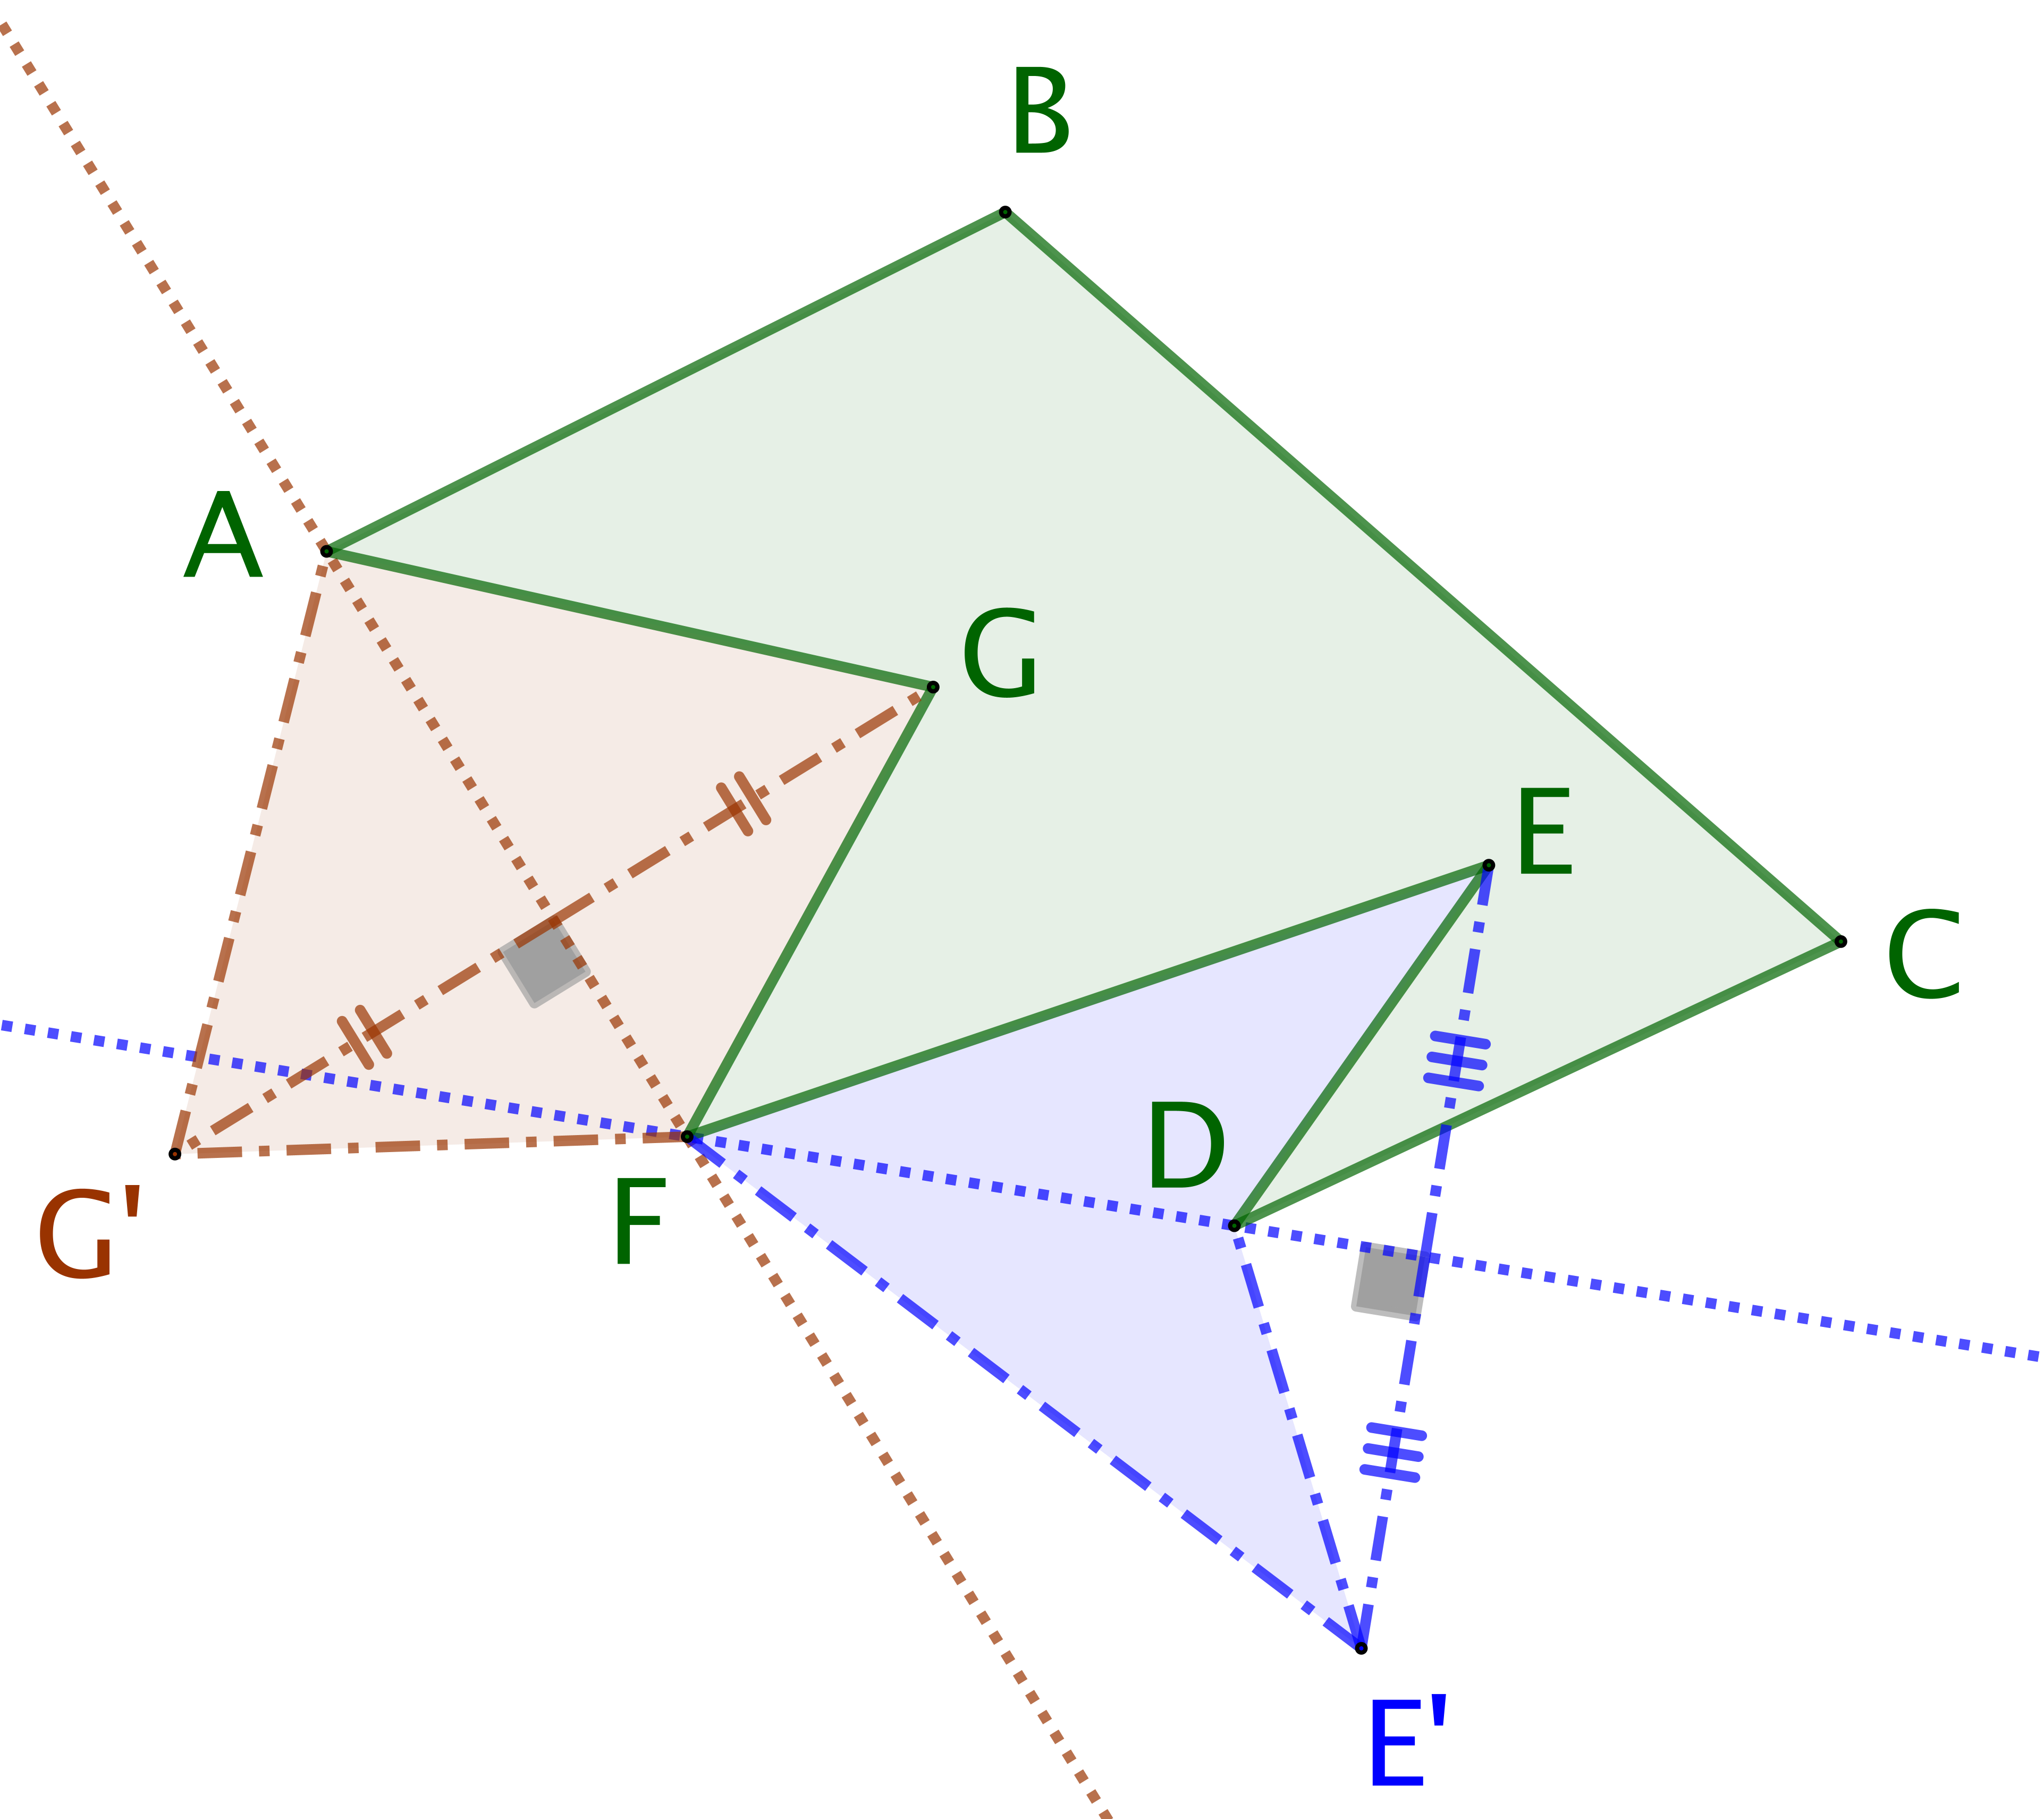
\includegraphics[scale=.4]{content/polygon/necessary-cond/non-convex-trap.png}
%	\end{center}
%
%
%	On peut aussi perdre des côtés lors de la construction comme dans l'exemple suivant où $C$, $D$ et $E^{\,\prime}$ sont alignés.%
%	\footnote{
%		Ce problème n'en est pas un. Une petite adaptation des arguments à venir permet de vérifier cela.
%	}
%
%	\begin{center}
%		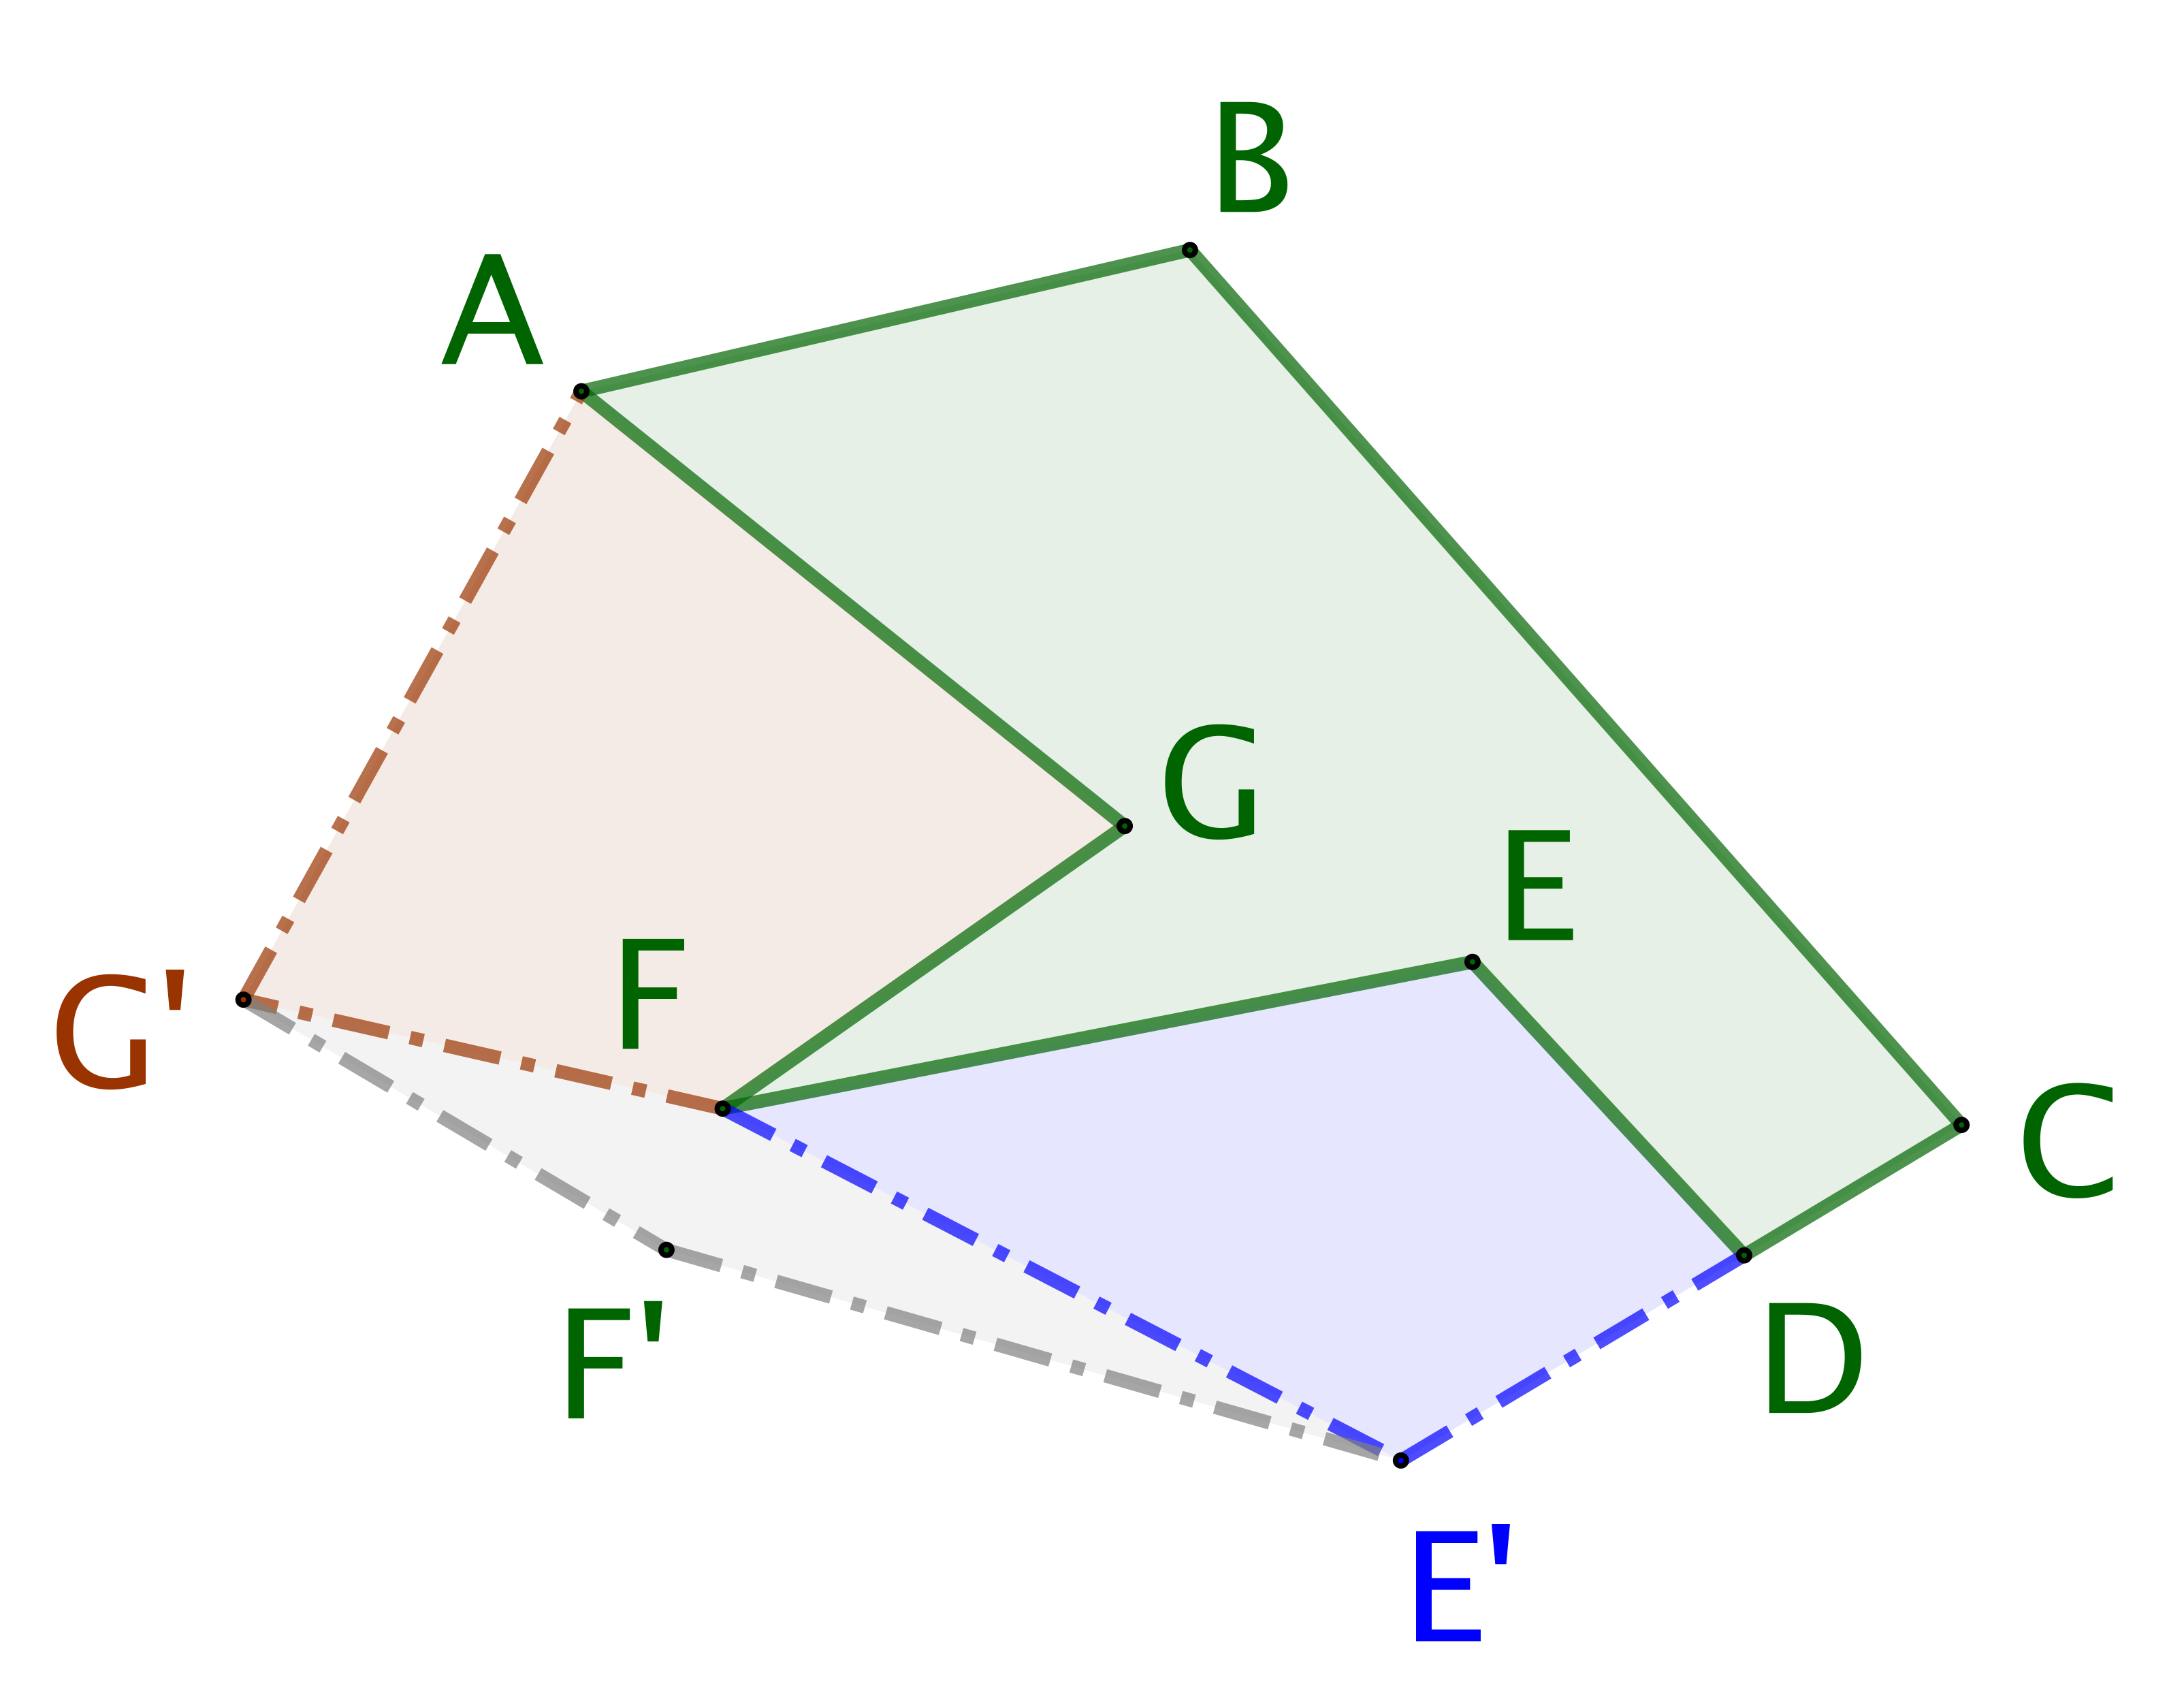
\includegraphics[scale=.4]{content/polygon/necessary-cond/non-convex-bad.png}
%	\end{center}
%
%
%	Laissons de côté la construction précédente pour nous concentrer sur la classique enveloppe convexe%
%	\footnote{
%		C'est le plus petit polygone convexe \og \emph{contenant} \fg\ le \ngone\ considéré, où \og \emph{petit} \fg\ est relatif à l'inclusion.
%	}
%	du \ngone\ de départ.
%	Par exemple, l'ennéagone $ABCDEFGHI$ non convexe ci-dessous admet le pentagone $ABDEG$ pour enveloppe convexe: le périmètre diminue et l'aire augmentent strictement, c'est très utile, mais il reste à avoir le bon nombre de côtés.
%
%	\begin{center}
%		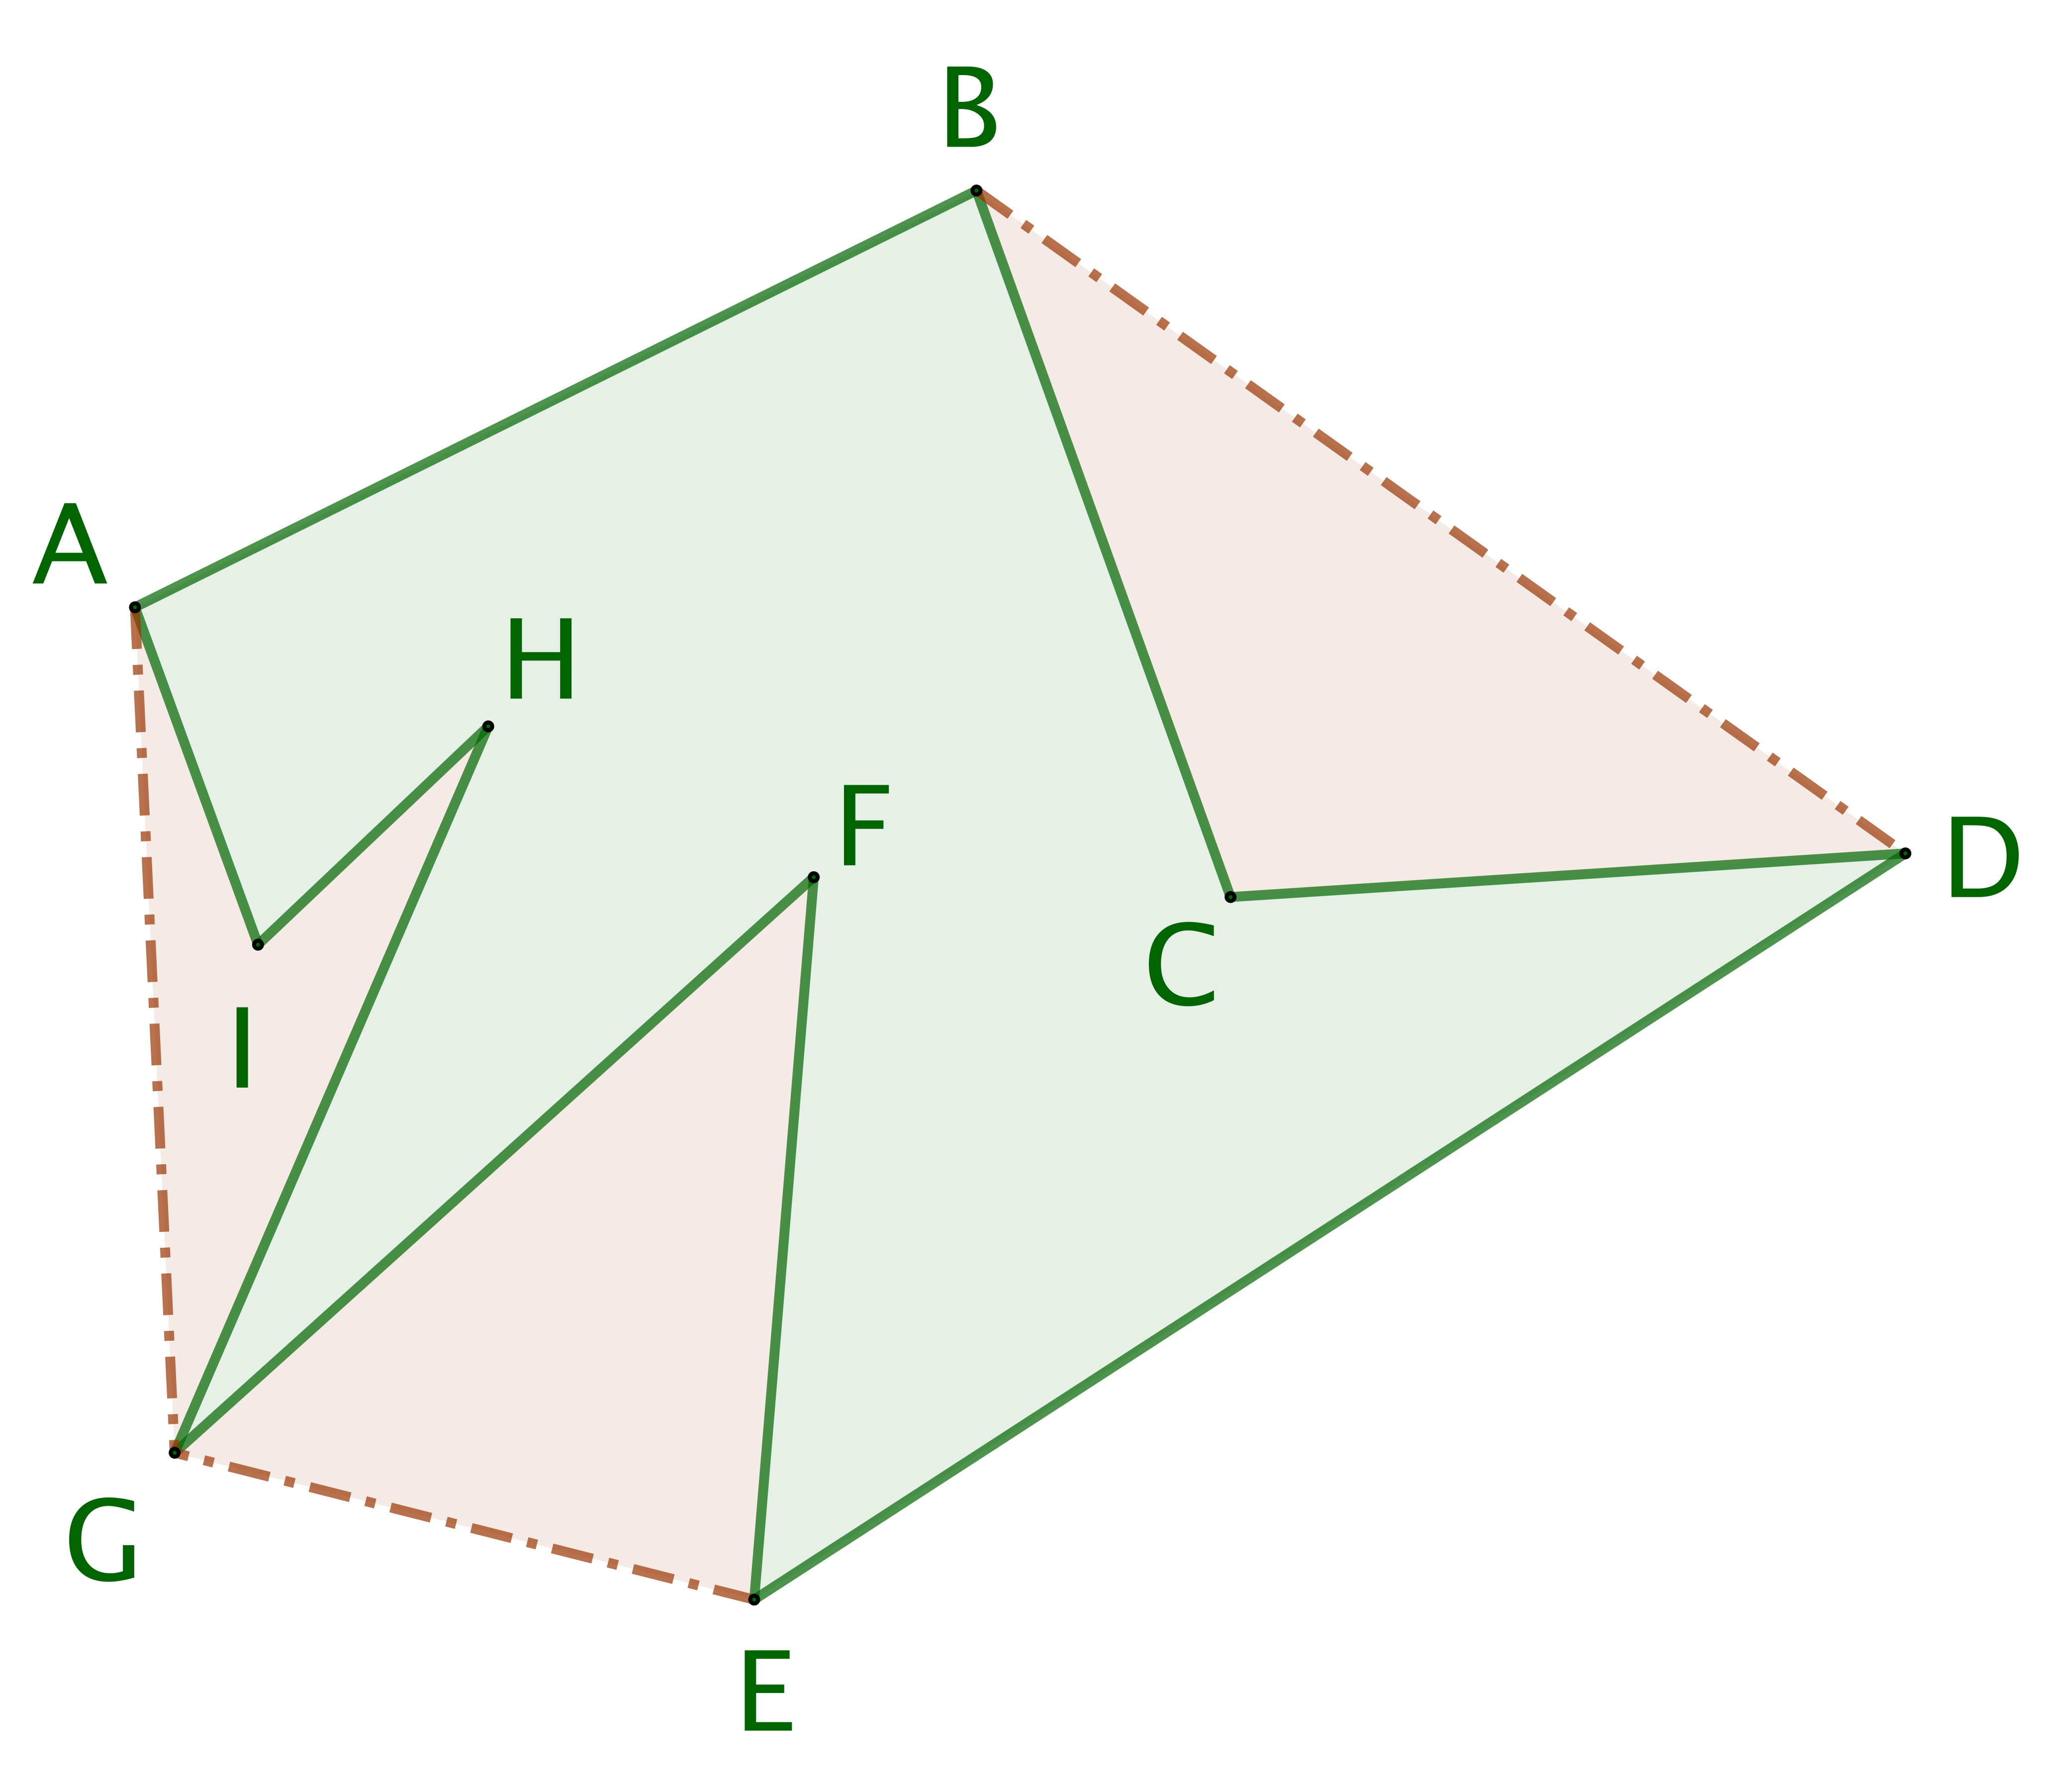
\includegraphics[scale=.4]{content/polygon/necessary-cond/convex-hull.png}
%	\end{center}
%
%	Une idée simple, que nous allons formaliser rigoureusement après, consiste à ajouter les sommets manquants suffisamment prêts des côtés de l'enveloppe convexe pour ne pas perdre la convexité, tout en gardant un périmètre inférieur strictement au périmètre initial, et une aire strictement plus grande que l'aire initiale. Si nous arrivons à faire ceci, alors une homothétie de rapport $r > 1$ nous ramènera au bon périmètre avec une aire strictement plus grande que l'aire initiale.
%	La figure suivante illustre cette idée.
%
%	\begin{center}
%		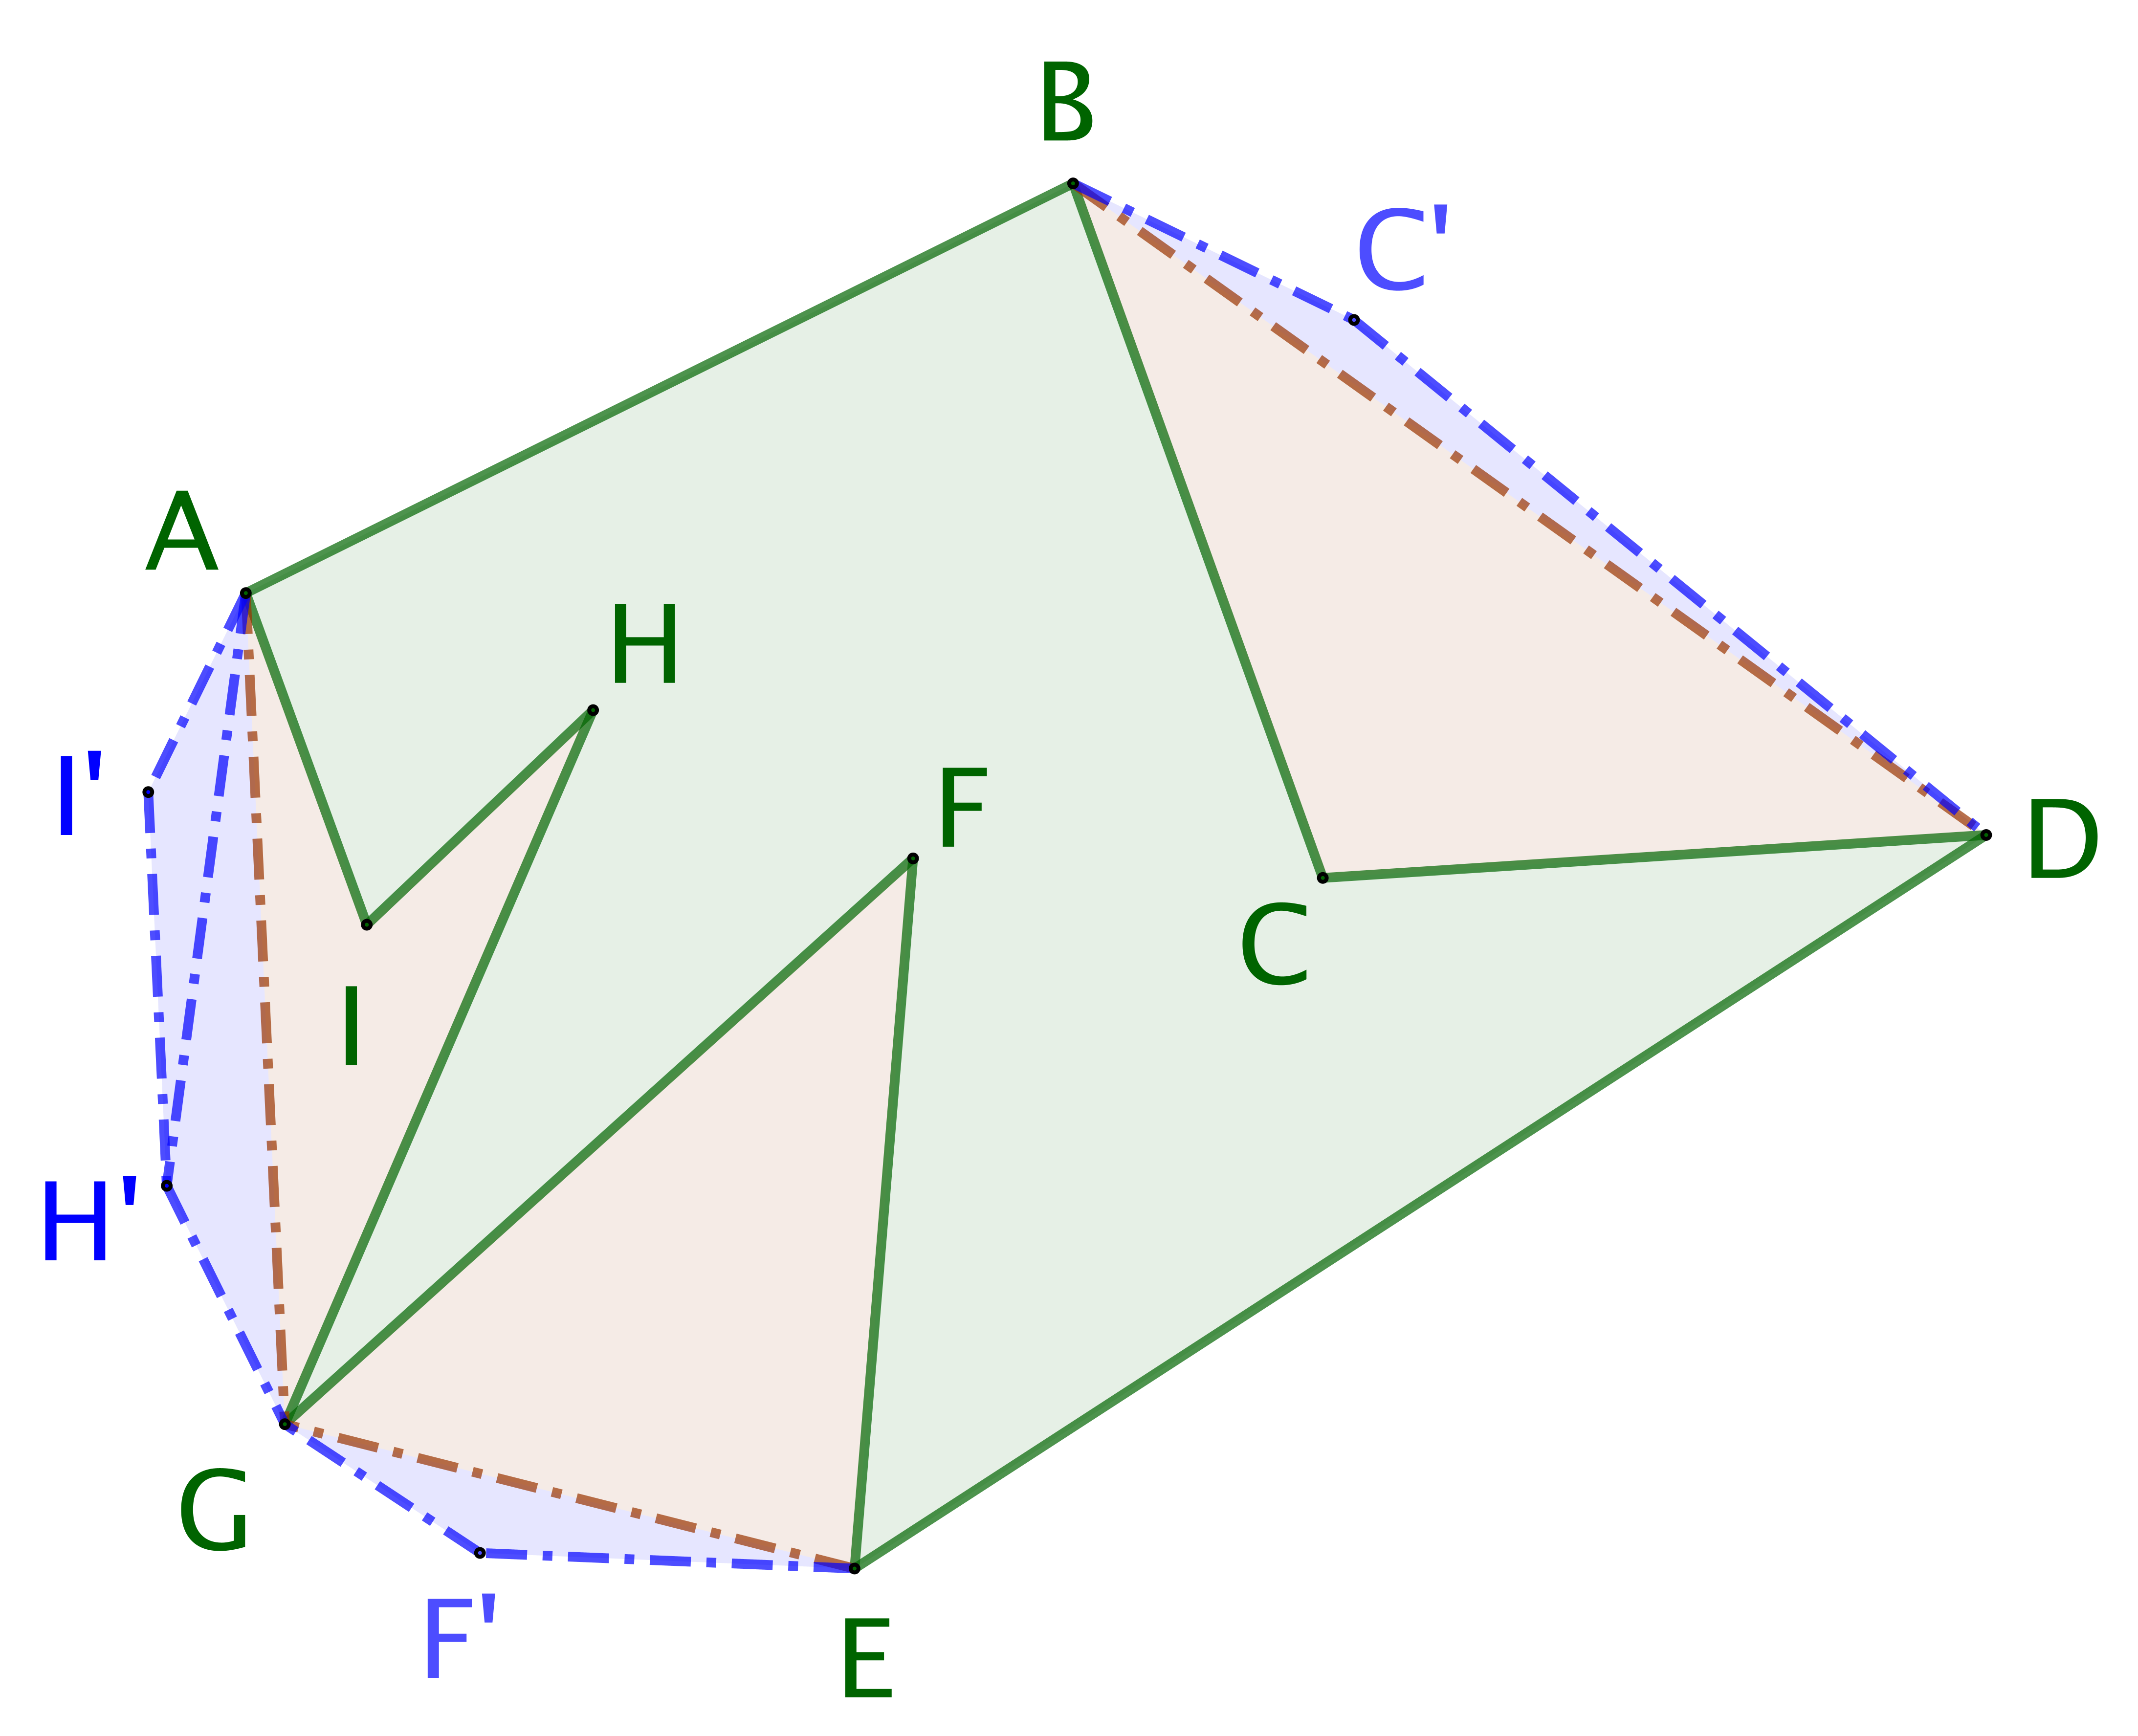
\includegraphics[scale=.4]{content/polygon/necessary-cond/convex-hull-distortion.png}
%	\end{center}
%
%
%	Considérons donc un \ngone\ non convexe $\setproba{P}$.
%	Son enveloppe convexe $\setproba{C}$ vérifie, par construction,
%	$\perim{\setproba{C}} < \perim{\setproba{P}}$
%	et
%	$\area{\setproba{C}} > \area{\setproba{P}}$.
%	Notons $m$ le nombre de sommets en moins dans $\setproba{C}$ relativement à $\setproba{P}$.
%	Si $m = 0$, il n'y a rien à faire.
%	Sinon, posons $\delta = \frac{\perim{\setproba{P}} - \perim{\setproba{C}}}{m}$.
%	%
%	\begin{enumerate}
%		\item \label{add-vertex-start}
%		Considérons $[AB]$ un côté quelconque de $\setproba{C}$.
%		Les droites portées par les côtés \og \emph{autour} \fg\ de $[AB]$ \og \emph{dessinent} \fg\ une région contenant toujours un triangle $ABC$ dont l'intérieur est à l'extérieur
%		\footnote{
%			C'est ce que l'on appelle de la \og \emph{low poetry} \fg\,.
%		}
%		de $\setproba{C}$ comme dans les deux cas ci-dessous.
%	%
%		\begin{multicols}{2}
%			\centering
%
%			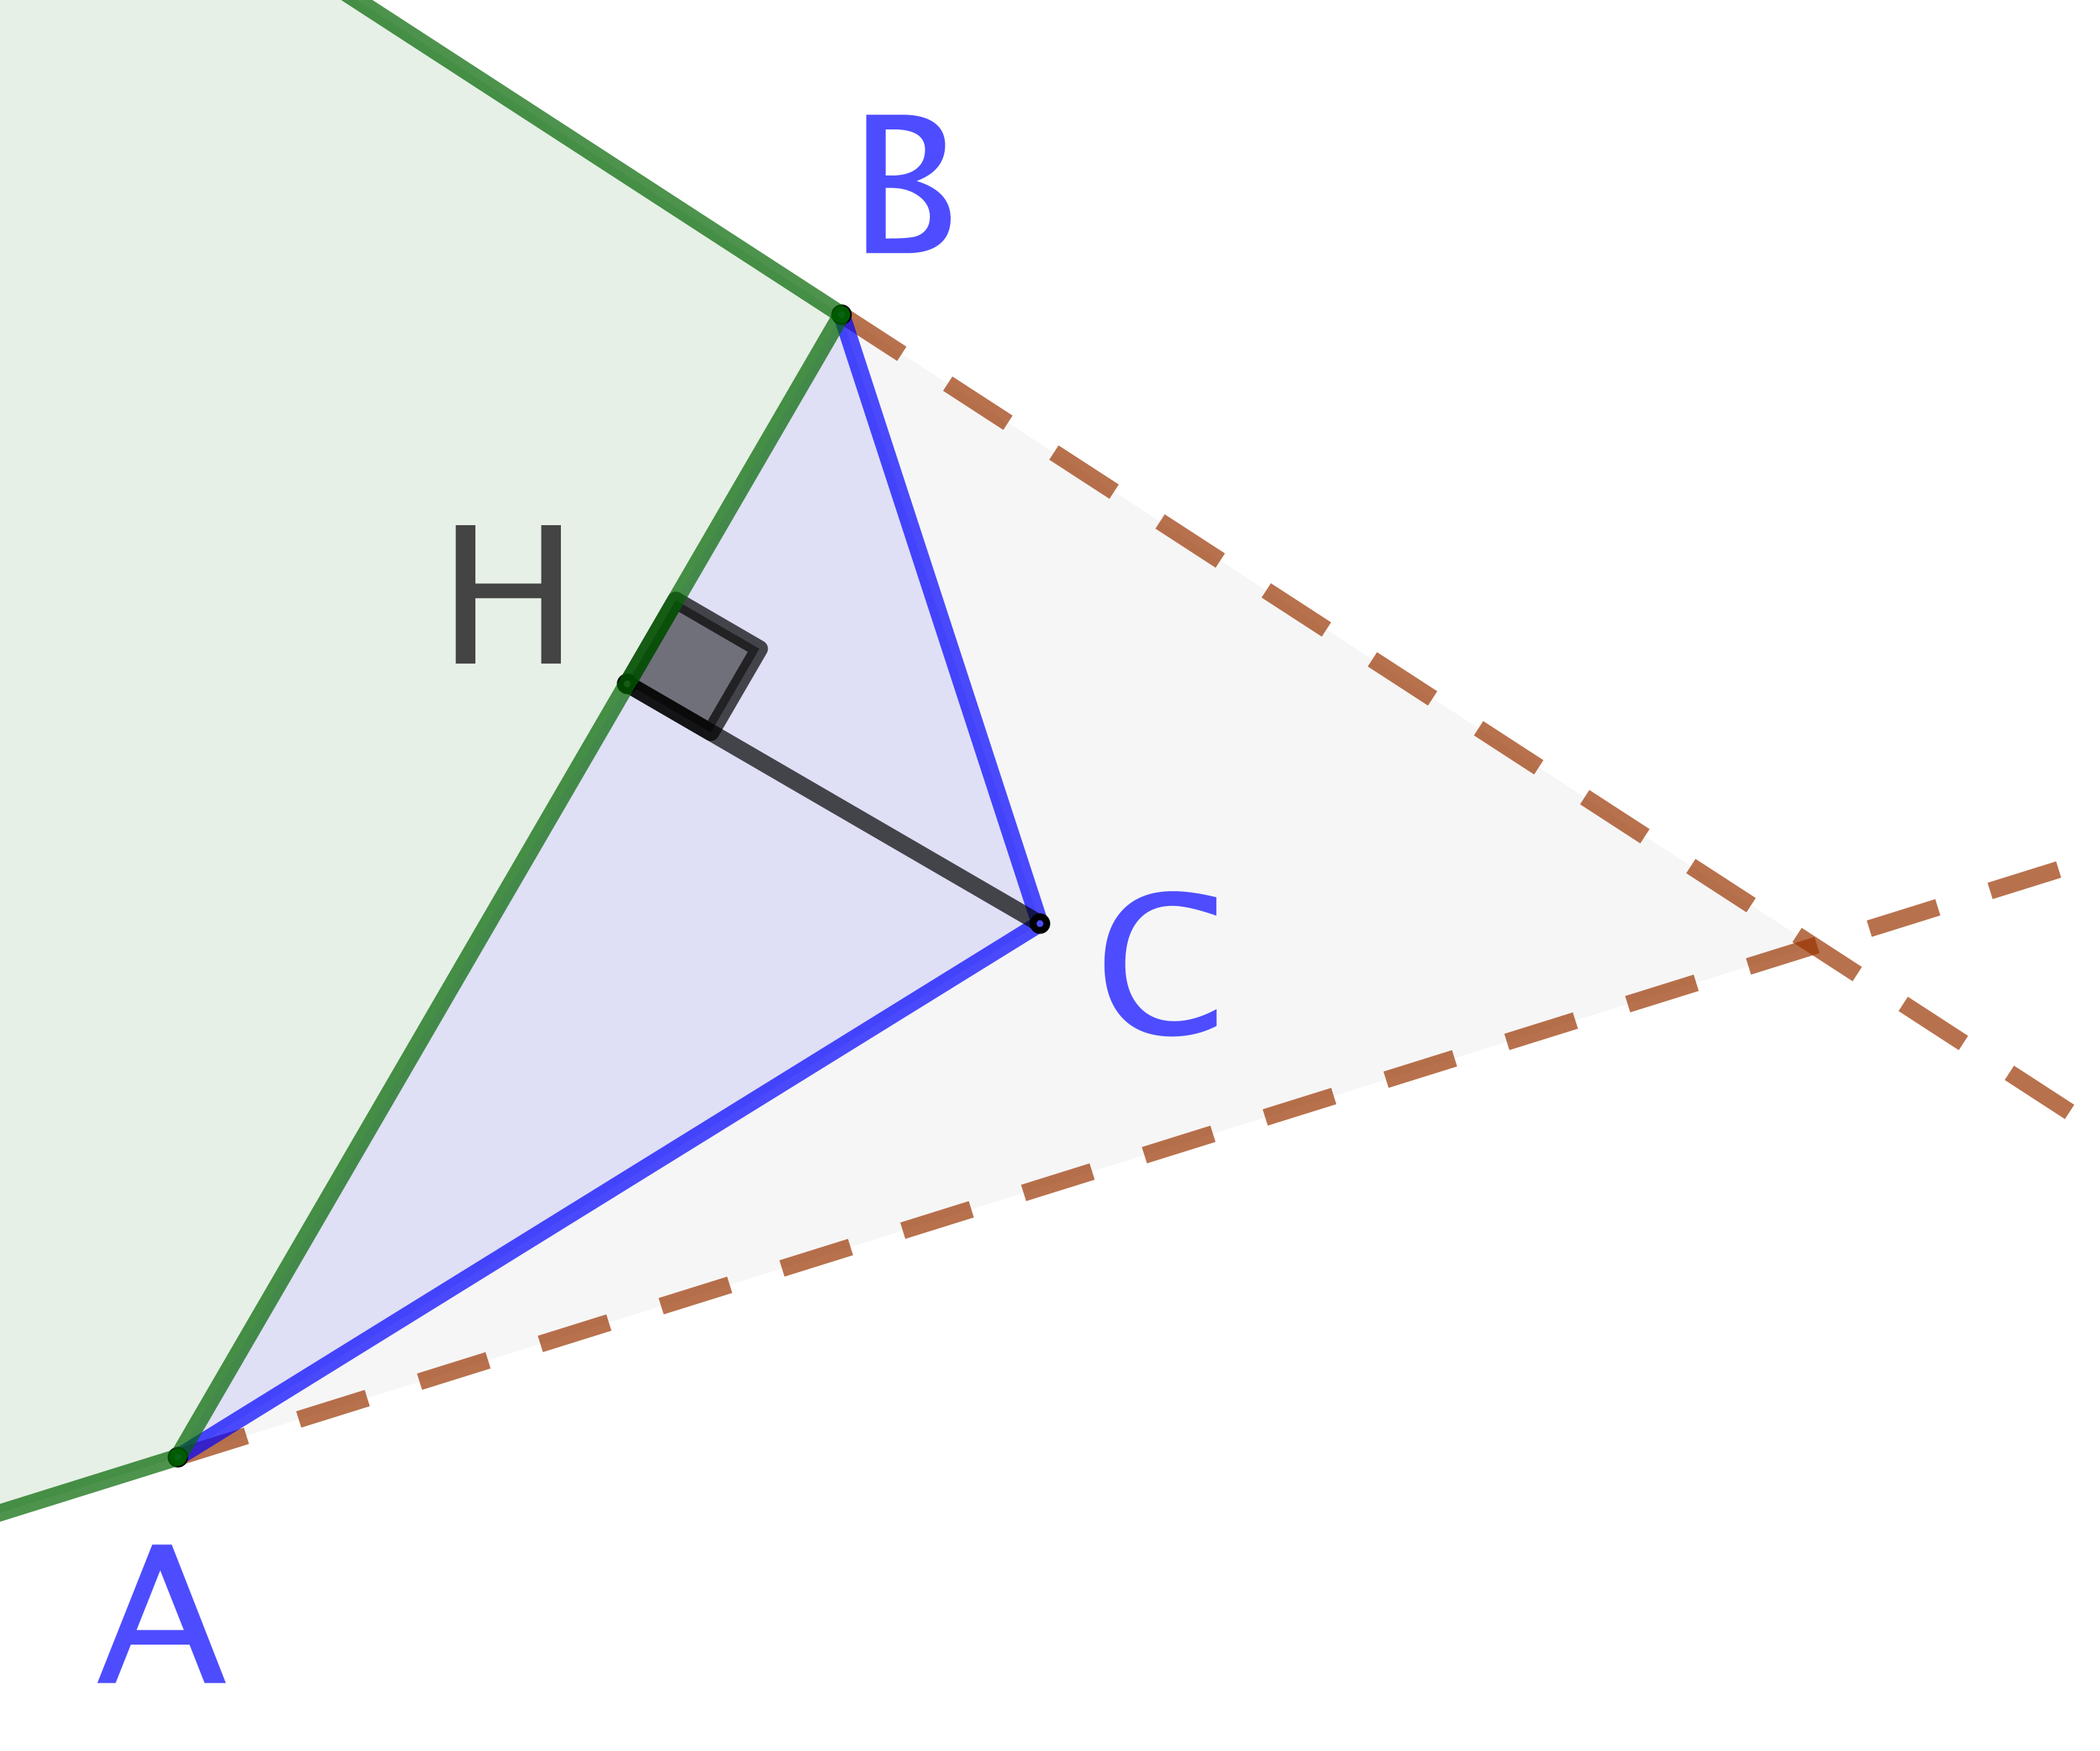
\includegraphics[scale=.4]{content/polygon/necessary-cond/add-vertex-1.png}
%
%			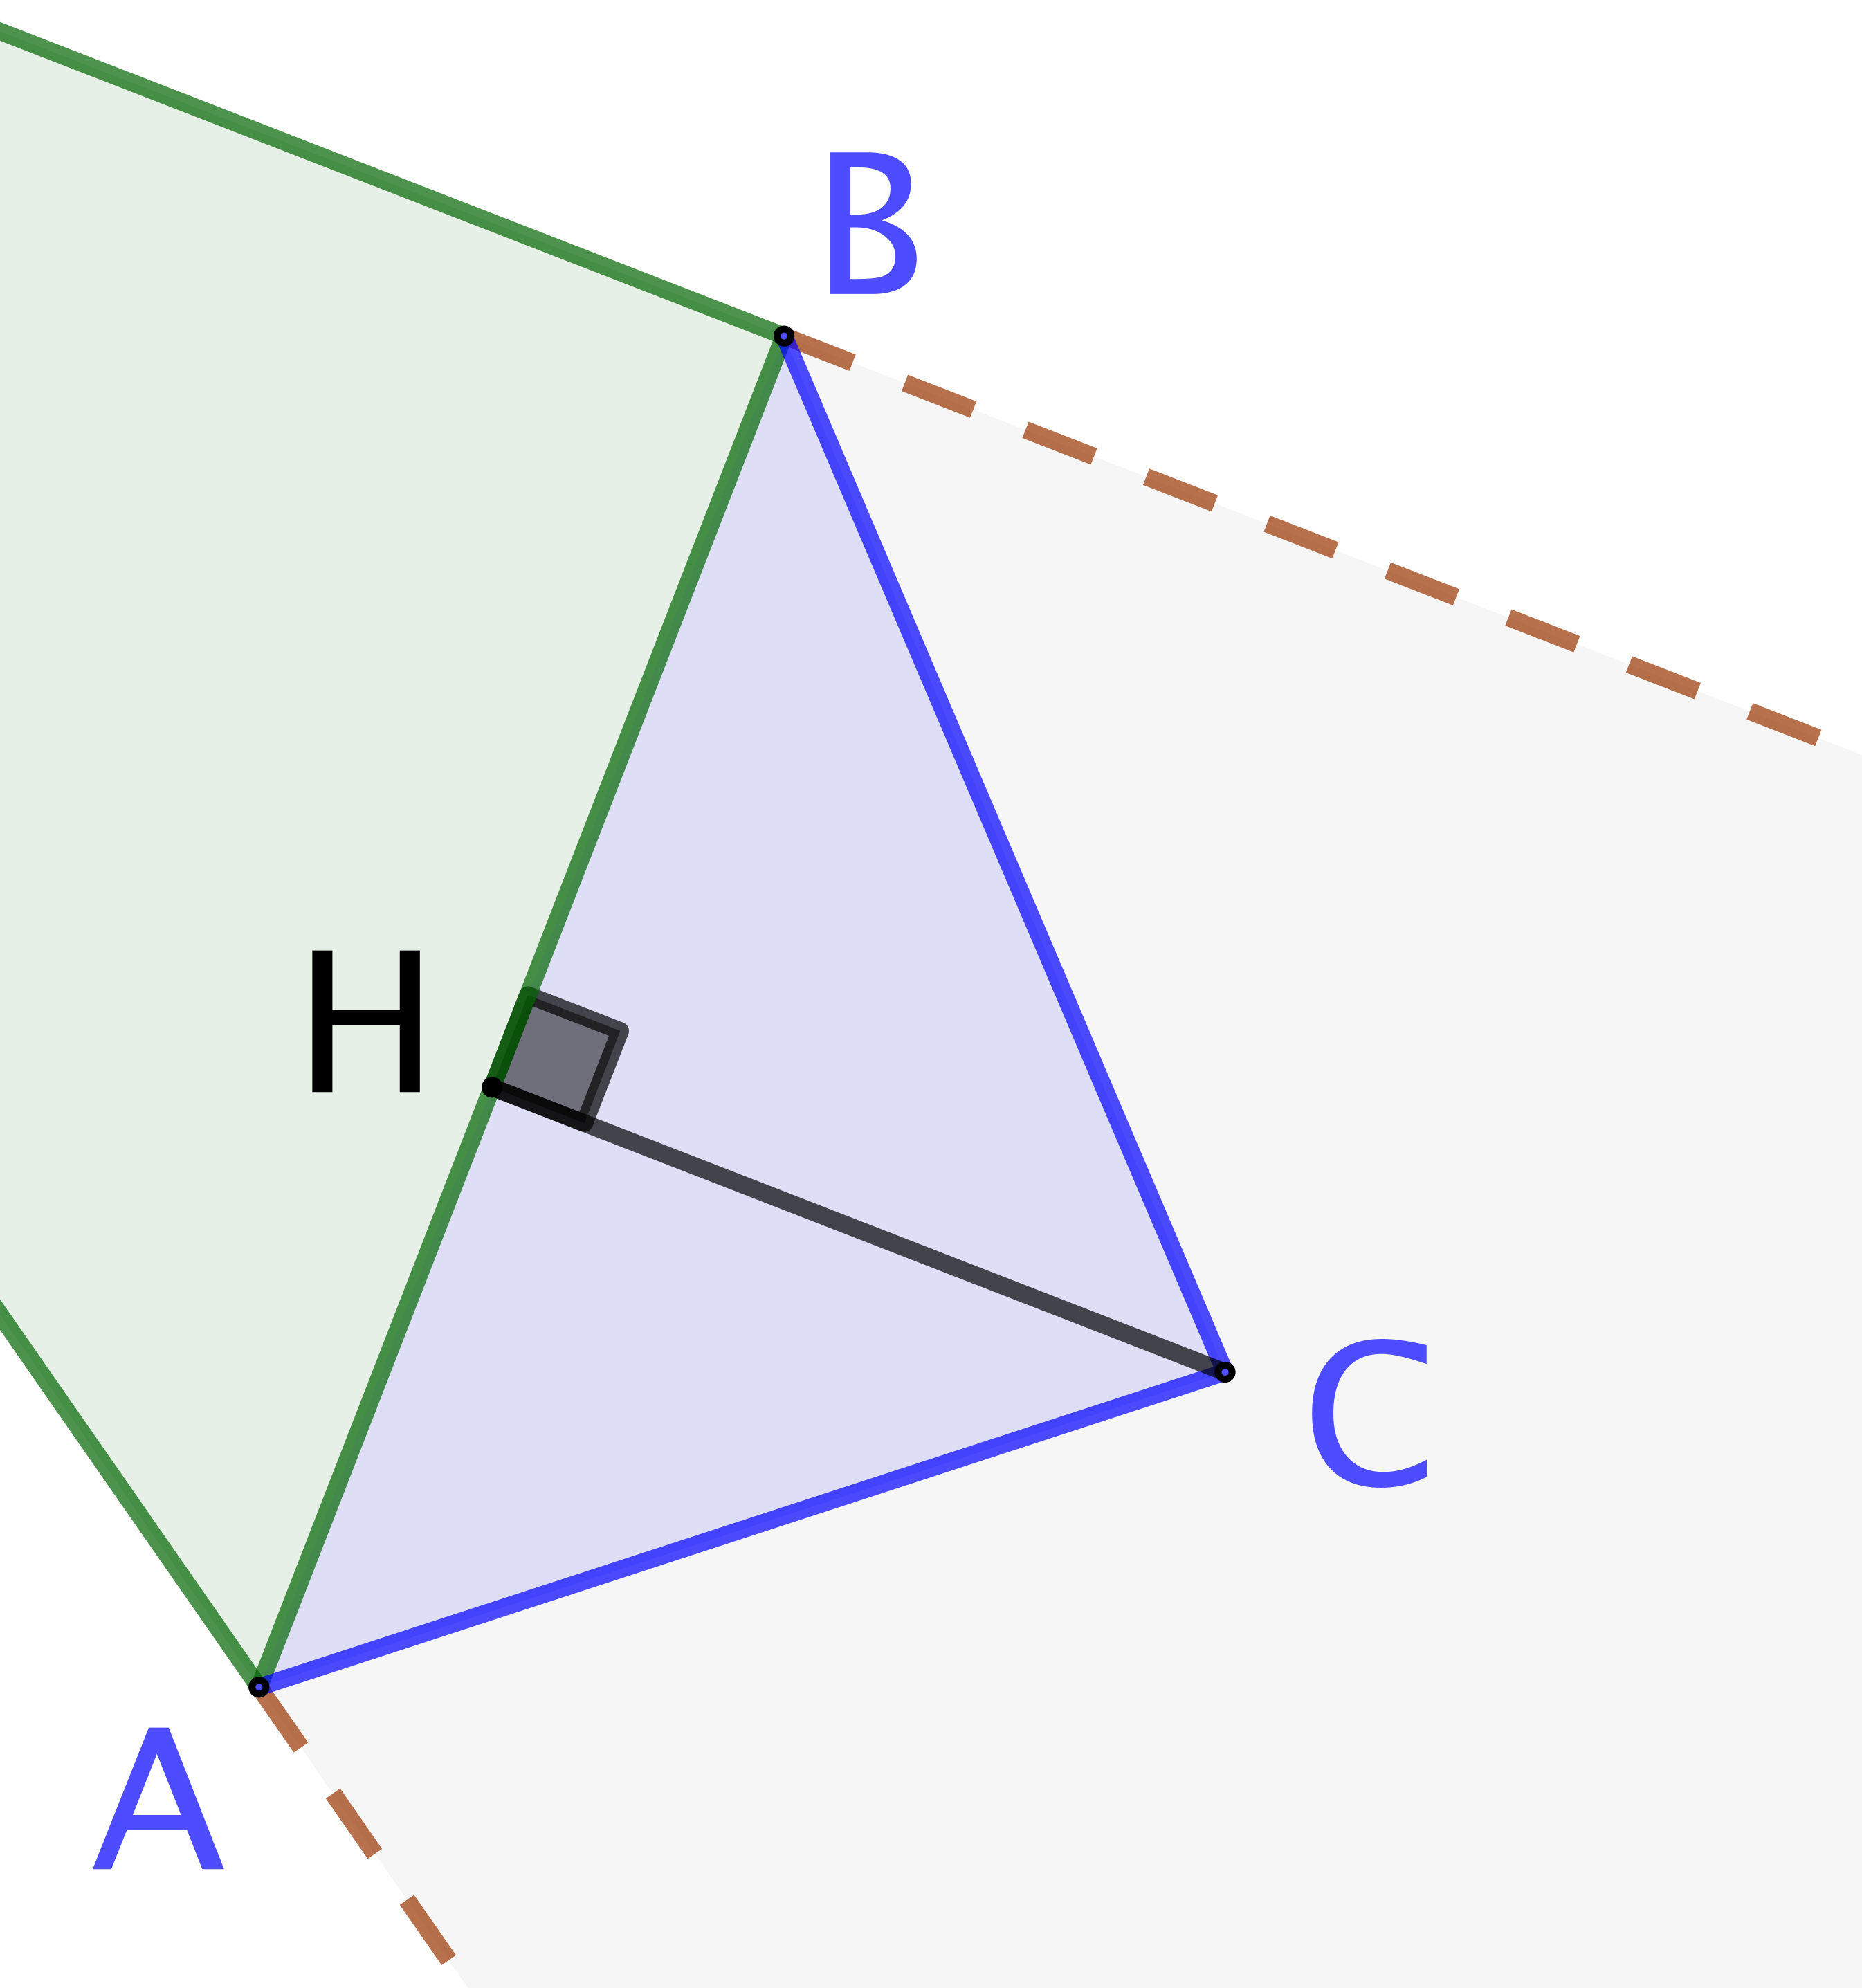
\includegraphics[scale=.4]{content/polygon/necessary-cond/add-vertex-2.png}
%		\end{multicols}
%
%		\item Clairement, le polygone $\setproba{C}^{\,\prime}$ obtenu à partir de $\setproba{C}$ en remplaçant le côté $[AB]$ par les côtés $[AC]$ et $[CB]$ est un convexe avec un sommet de plus que $\setproba{C}$.
%
%		\item \label{add-vertex-end}
%		Comme $HC$ peut être rendu aussi proche de $0$ que souhaité, il est aisé de voir que l'on peut choisir cette distance de sorte que $AC + BC < AB + \delta$.
%		Dès lors, le périmètre de $\setproba{C}^{\,\prime}$ augmente inférieurement à $\delta$ relativement à $\setproba{C}$.
%
%		\item En répétant $(m-1)$ fois les étapes \ref{add-vertex-start} à \ref{add-vertex-end}, nous obtenons un \ngone\ convexe $\setproba{P}^{\,\prime}$ tel que
%		$\area{\setproba{P}^{\,\prime}} > \area{\setproba{P}}$
%		et
%		$\perim{\setproba{P}^{\,\prime}} < \perim{\setproba{C}} + m \delta = \perim{\setproba{P}}$.
%	\end{enumerate}
%\end{proof}
%
%
%\begin{remark}
%	Le fait précédent permet de toujours se ramener au cas d'un \ngone\ convexe.
%\end{remark}
%
%
%% ----------------------- %
%
%
%\begin{fact} \label{iso-poly}
%	Si un \ngone\ convexe $\setproba{P}$ n'est pas un \nequi, alors on peut construire un \ngone\ convexe $\setproba{P}^{\,\prime}$ tel que
%	$\perim{\setproba{P}^{\,\prime}} = \perim{\setproba{P}}$
%	et
%	$\area{\setproba{P}^{\,\prime}} > \area{\setproba{P}}$.
%\end{fact}
%
%
%\begin{proof}
%	Considérons un \ngone\ convexe $\setproba{P}$ qui ne soit pas un \nequi.
%	Dans ce cas, $\setproba{P}$ admet un triplet de sommets consécutifs $A$, $B$ et $C$ tels que $AB \neq BC$ (sinon, on obtiendrait de proche en proche un \nequi).
%	La construction vue dans la preuve du fait \ref{tri-one-side-fixed} nous donne la solution: voir les deux dessins ci-après dans lesquels $(AC) \parallel (BB^{\,\prime})$.
%	Pour le 2\ieme\ cas, il n'est pas possible d'utiliser le triangle $AB^{\,\prime}C$ isocèle en $B^{\,\prime}$ car $(B^{\,\prime}C)$ porte le côté de $\setproba{P}$ de sommet $C$ juste après $[BC]$, mais ce problème se contourne en considérant un point $B^{\,\prime\prime}$ de $]BB^{\,\prime}[$.
%	%
%	\begin{multicols}{2}
%		\centering
%
%		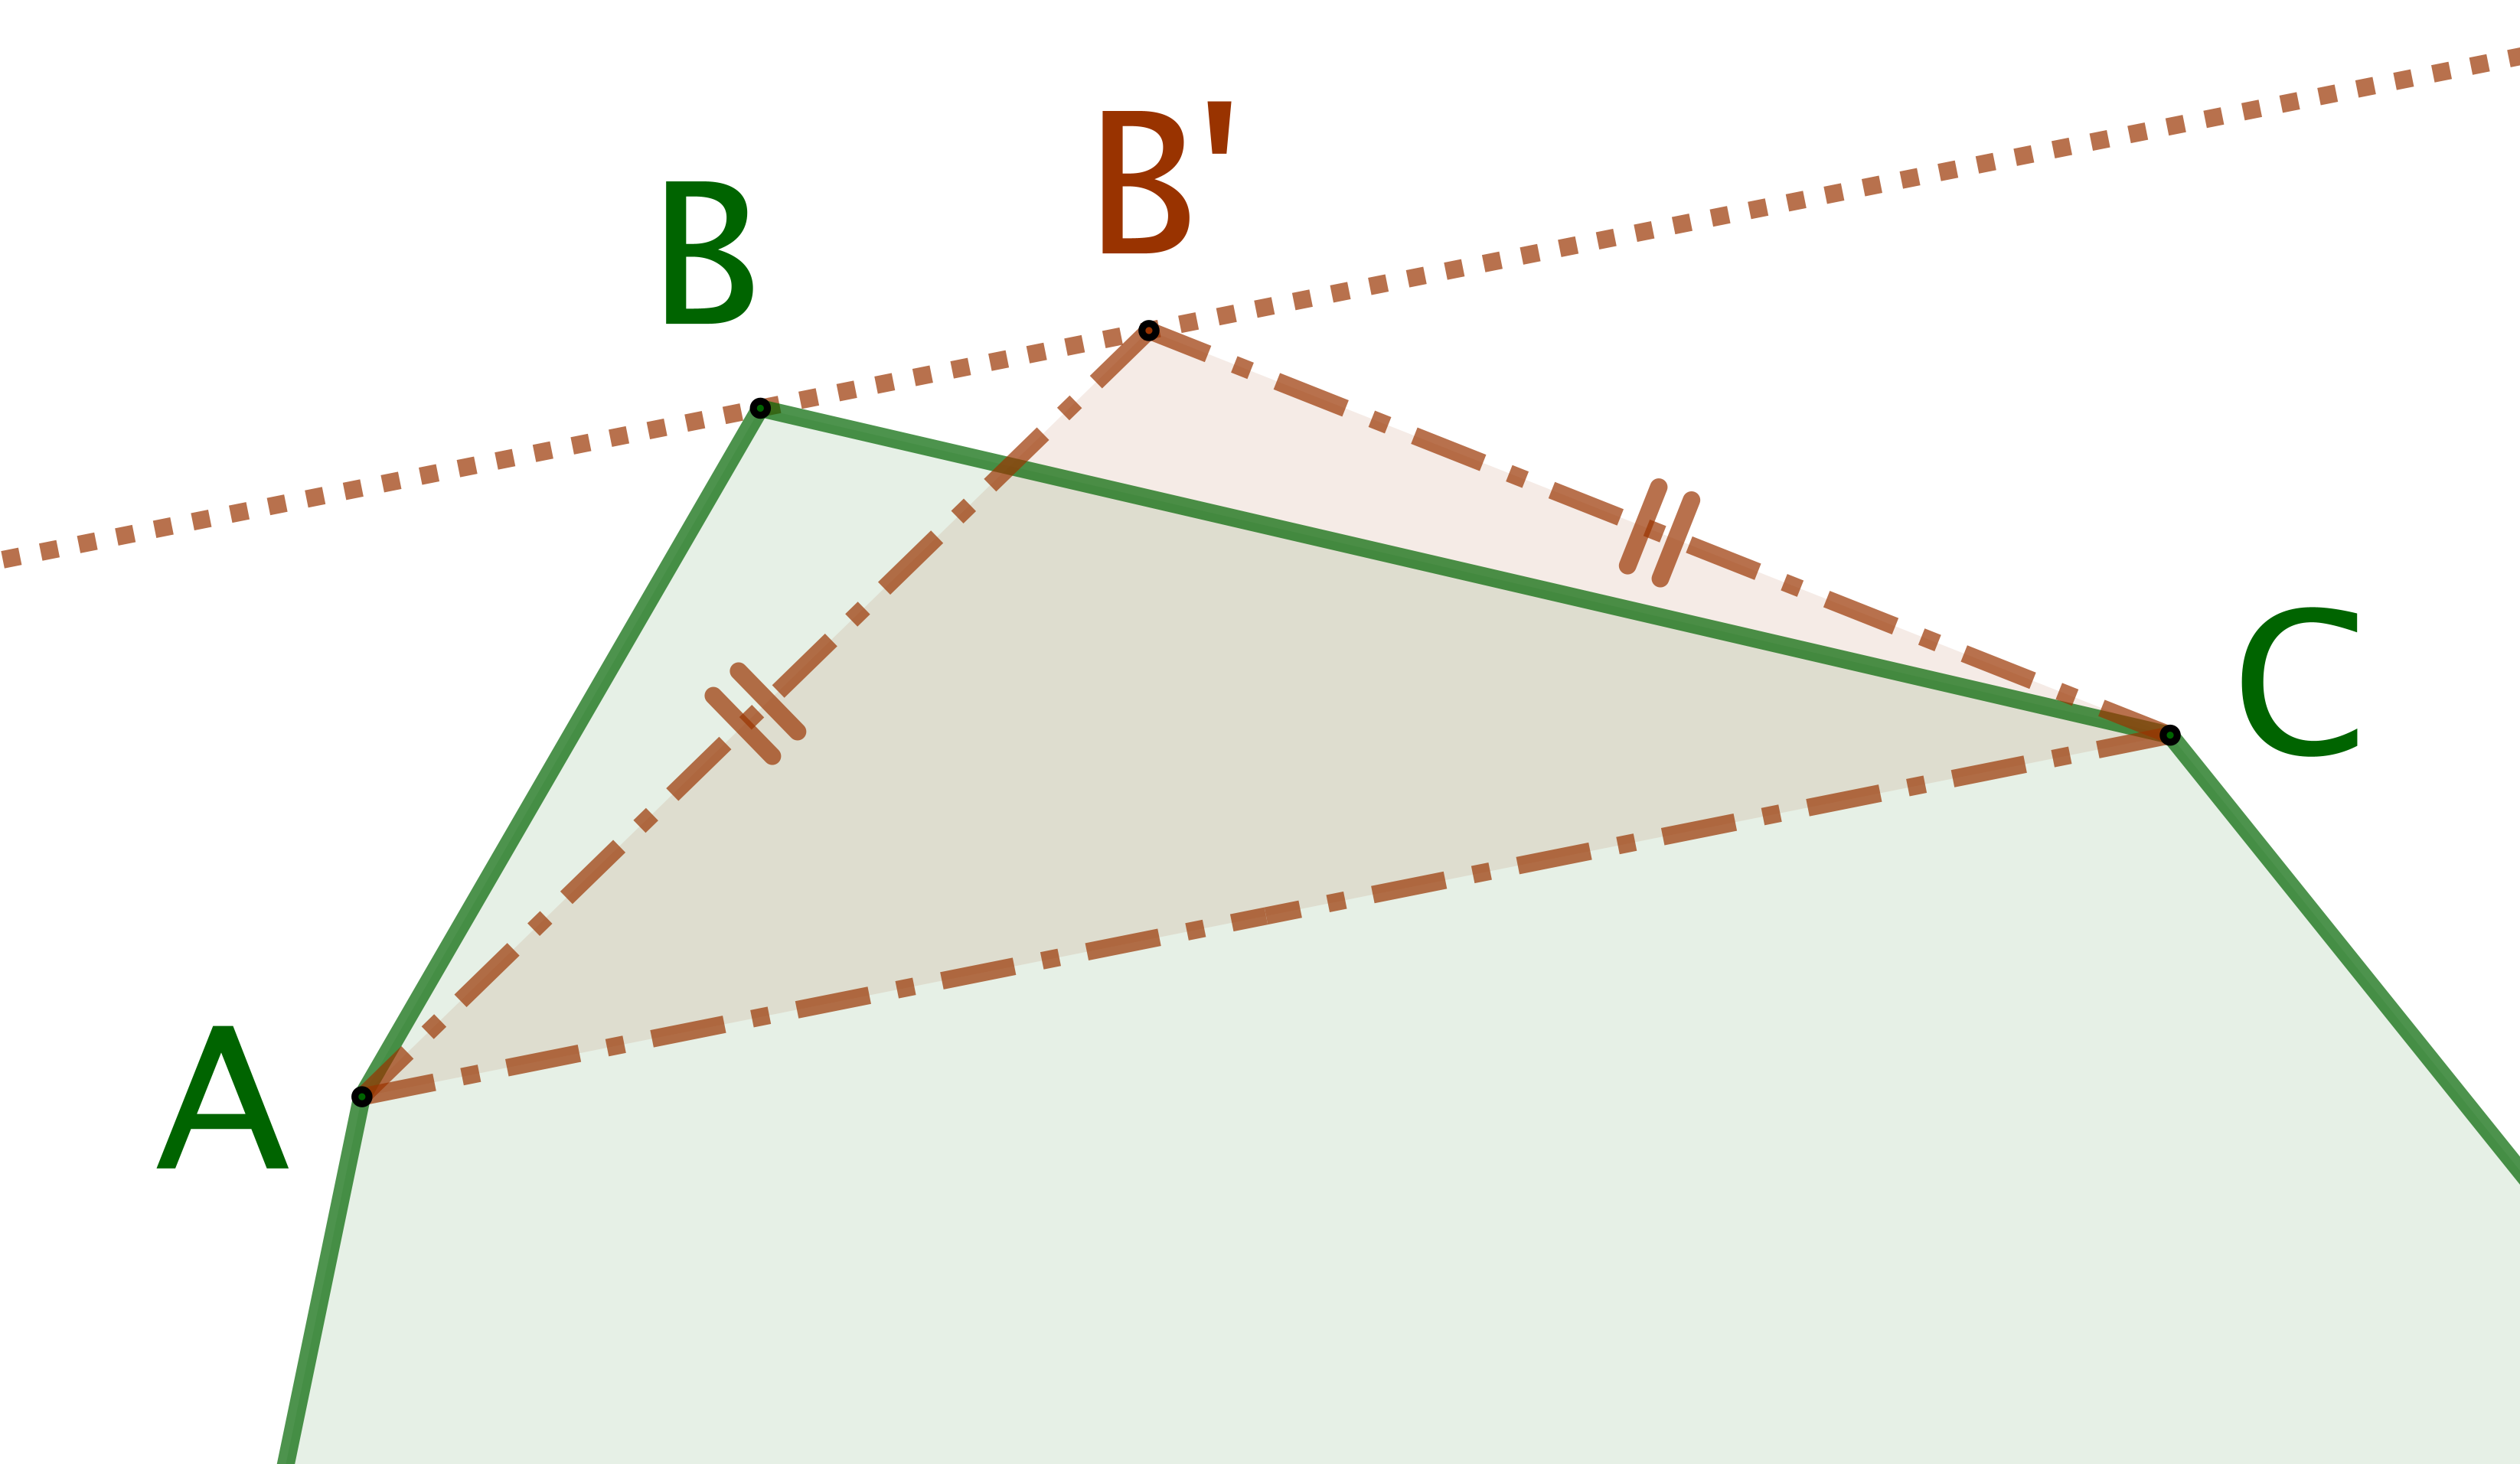
\includegraphics[scale=.4]{content/polygon/necessary-cond/not-iso-OK.png}
%
%		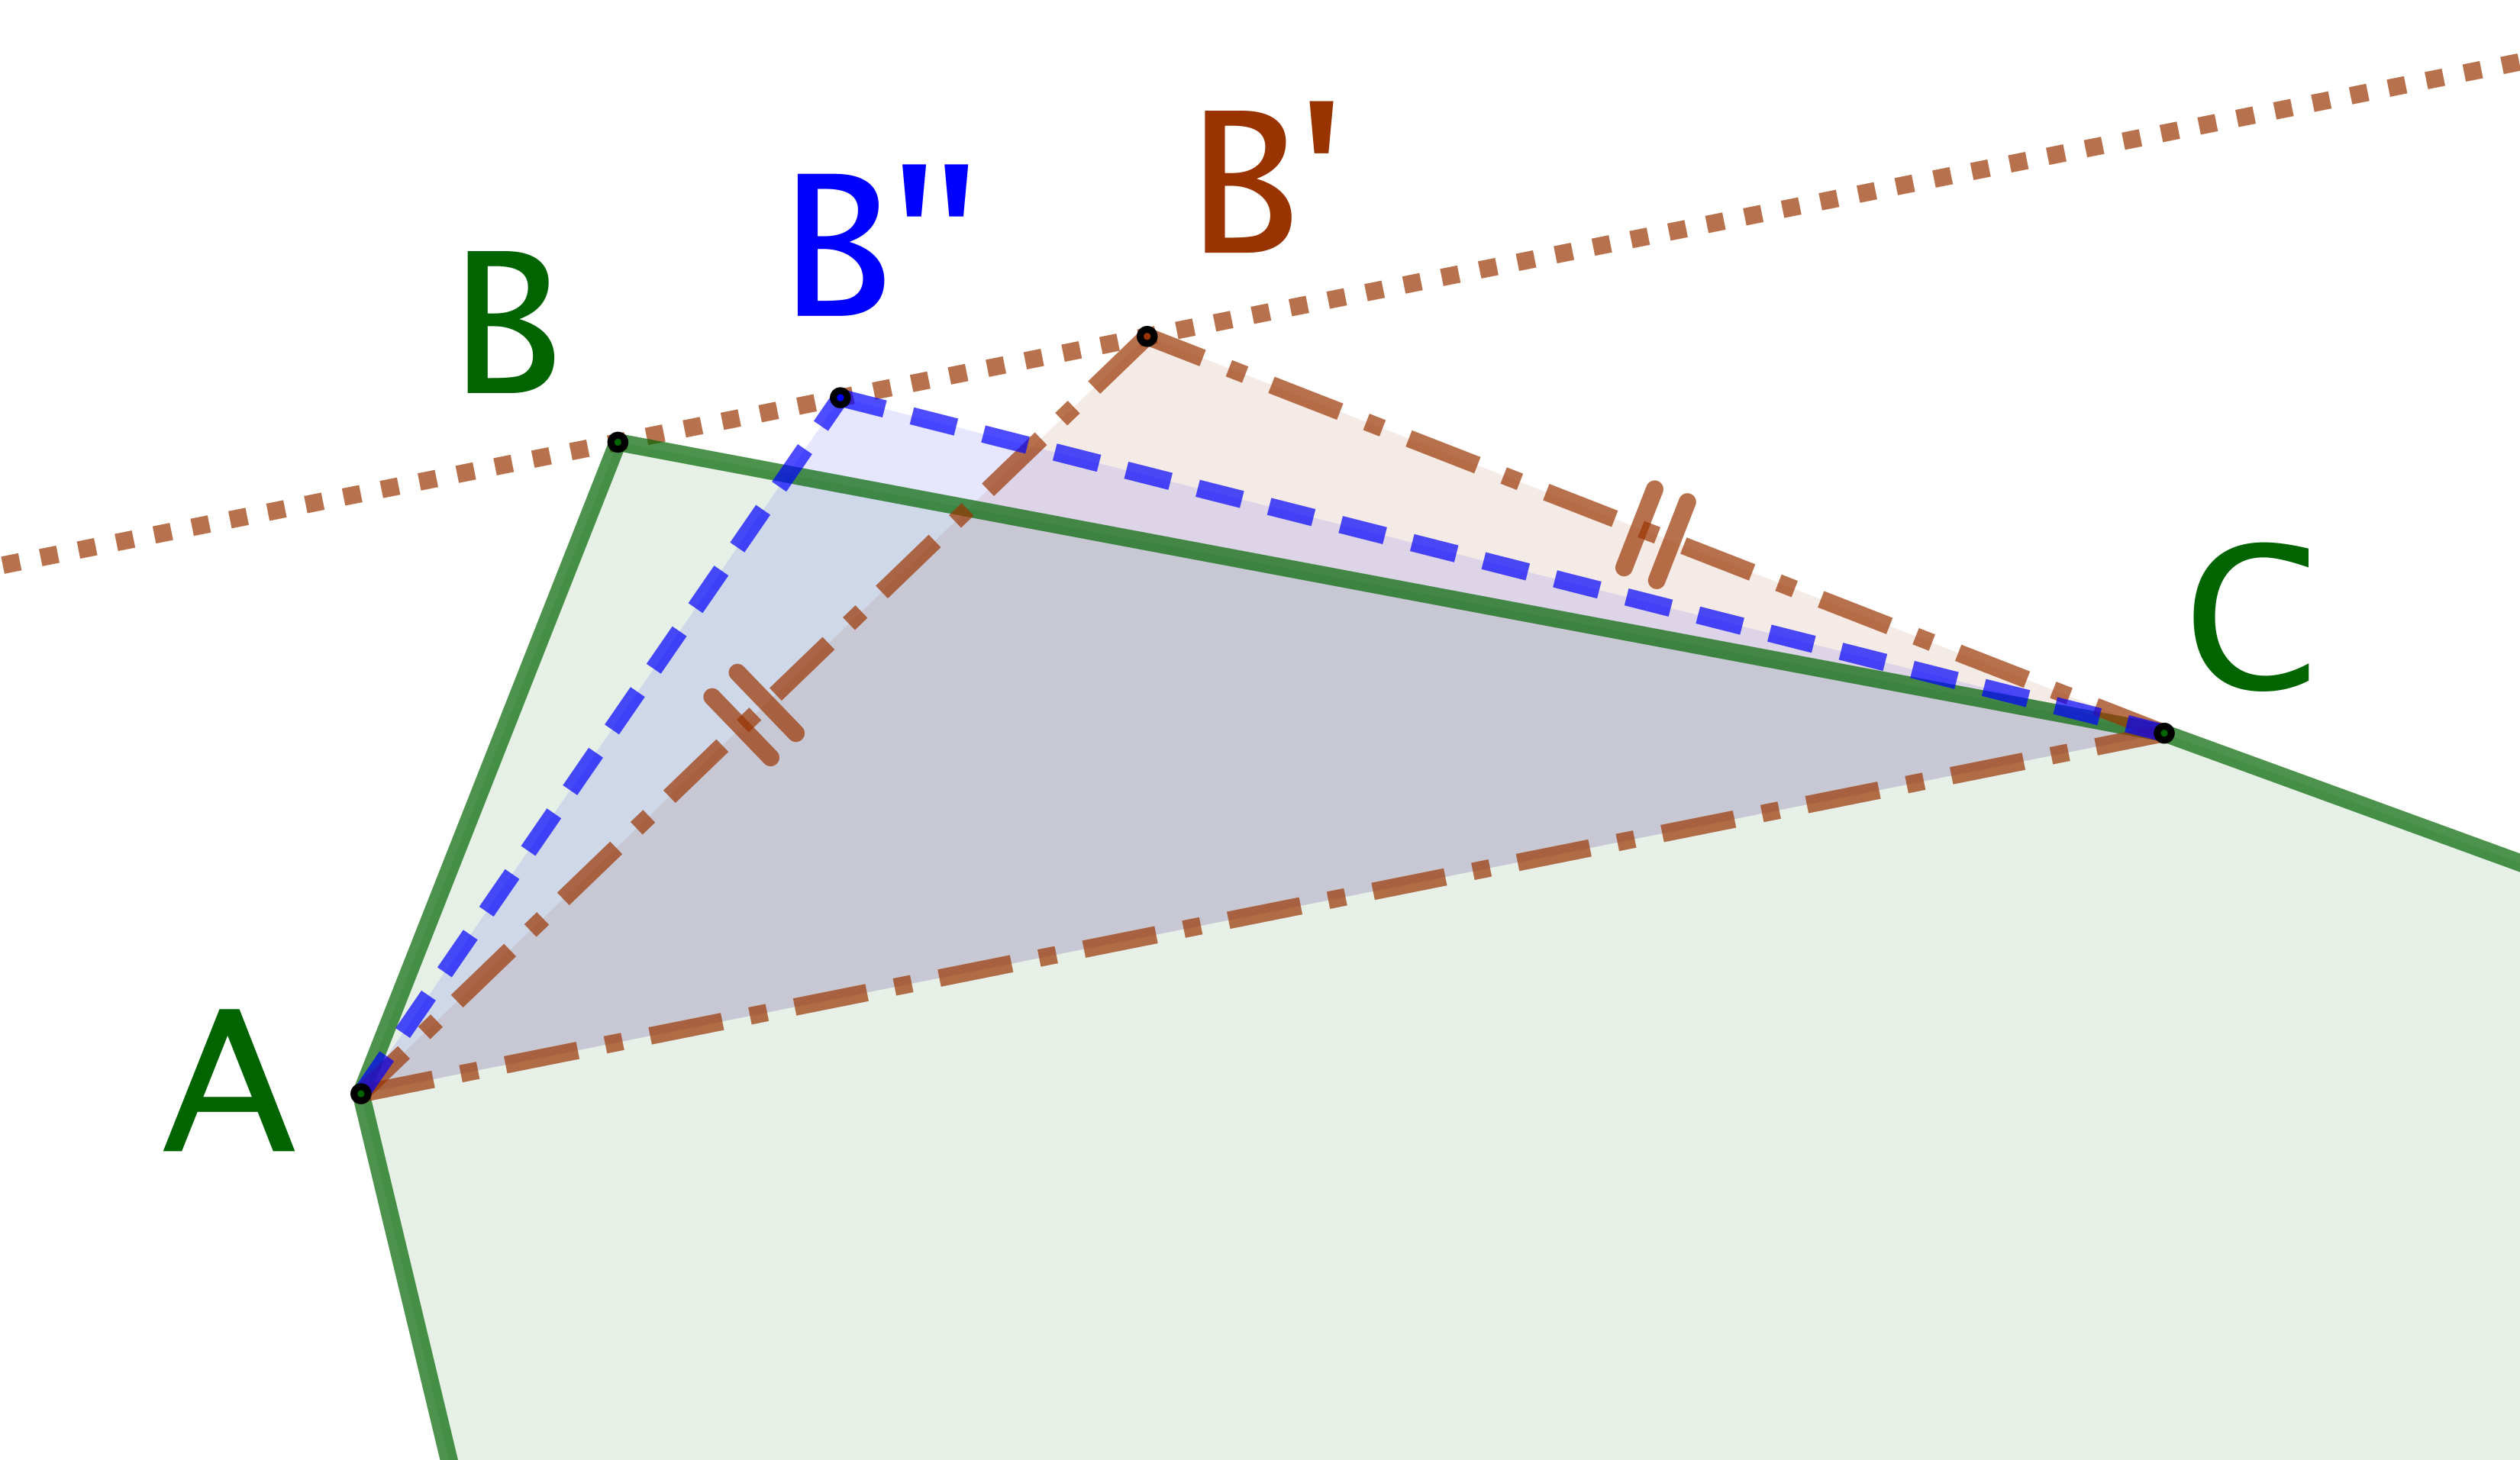
\includegraphics[scale=.4]{content/polygon/necessary-cond/not-iso-KO.png}
%	\end{multicols}
%
%	Dans chaque cas, nous avons construit un \ngone\ convexe $\setproba{P}^{\,\prime\prime}$ tel que
%	$\perim{\setproba{P}^{\,\prime\prime}} < \perim{\setproba{P}}$
%	et
%	$\area{\setproba{P}^{\,\prime\prime}} = \area{\setproba{P}}$.
%	Un simple agrandissement donne un \ngone\ convexe $\setproba{P}^{\,\prime}$ vérifiant
%	$\perim{\setproba{P}^{\,\prime}} = \perim{\setproba{P}}$
%	et
%	$\area{\setproba{P}^{\,\prime}} > \area{\setproba{P}}$.
%\end{proof}
%
%
\newpage  % TEMPO

\begin{remark}
	Le fait précédent ne permet pas de se ramener toujours au cas d'un \nequi\ convexe. Il nous dit juste que si un \ngone\ convexe maximise son aire à périmètre fixé, alors il devra être un \nequi. La nuance est importante, et une similaire existe pour le fait suivant.
\end{remark}


% ----------------------- %


\begin{fact} \label{almost-reg-poly}
	Si un \nequi\ convexe $\setproba{P}$ n'est pas un \niso,
	alors il existe un \ngone\ convexe $\setproba{P}^{\,\prime}$ tel que
	$\perim{\setproba{P}^{\,\prime}} = \perim{\setproba{P}}$
	et
	$\area{\setproba{P}^{\,\prime}} > \area{\setproba{P}}$.
\end{fact}


\begin{proof}
	SCHÉMA AVEC CÔTÉ CONTIGUS CAR AU FINAL PAS SI SIMPLE PUISUQ'UN COTÉ PEUT ETRE MANGÉ
	c'est toujours omis !
	
	PARLER DE Zenodore ais trop long et peu éclaiant avec aussi le problème du côté mangé !!!
	
	la preuve geo est trop longue, donc ici on accepte l'analyse !
	
	Par hypothèse, nous avons deux paires de côtés
	$\big( [AB] , [BC] \big)$ et
	$\big( [EF] , [FG] \big)$ tels que
	$\anglein{BAC} < \anglein{FEG}$ comme ci-dessous.
	%
	\begin{center}
		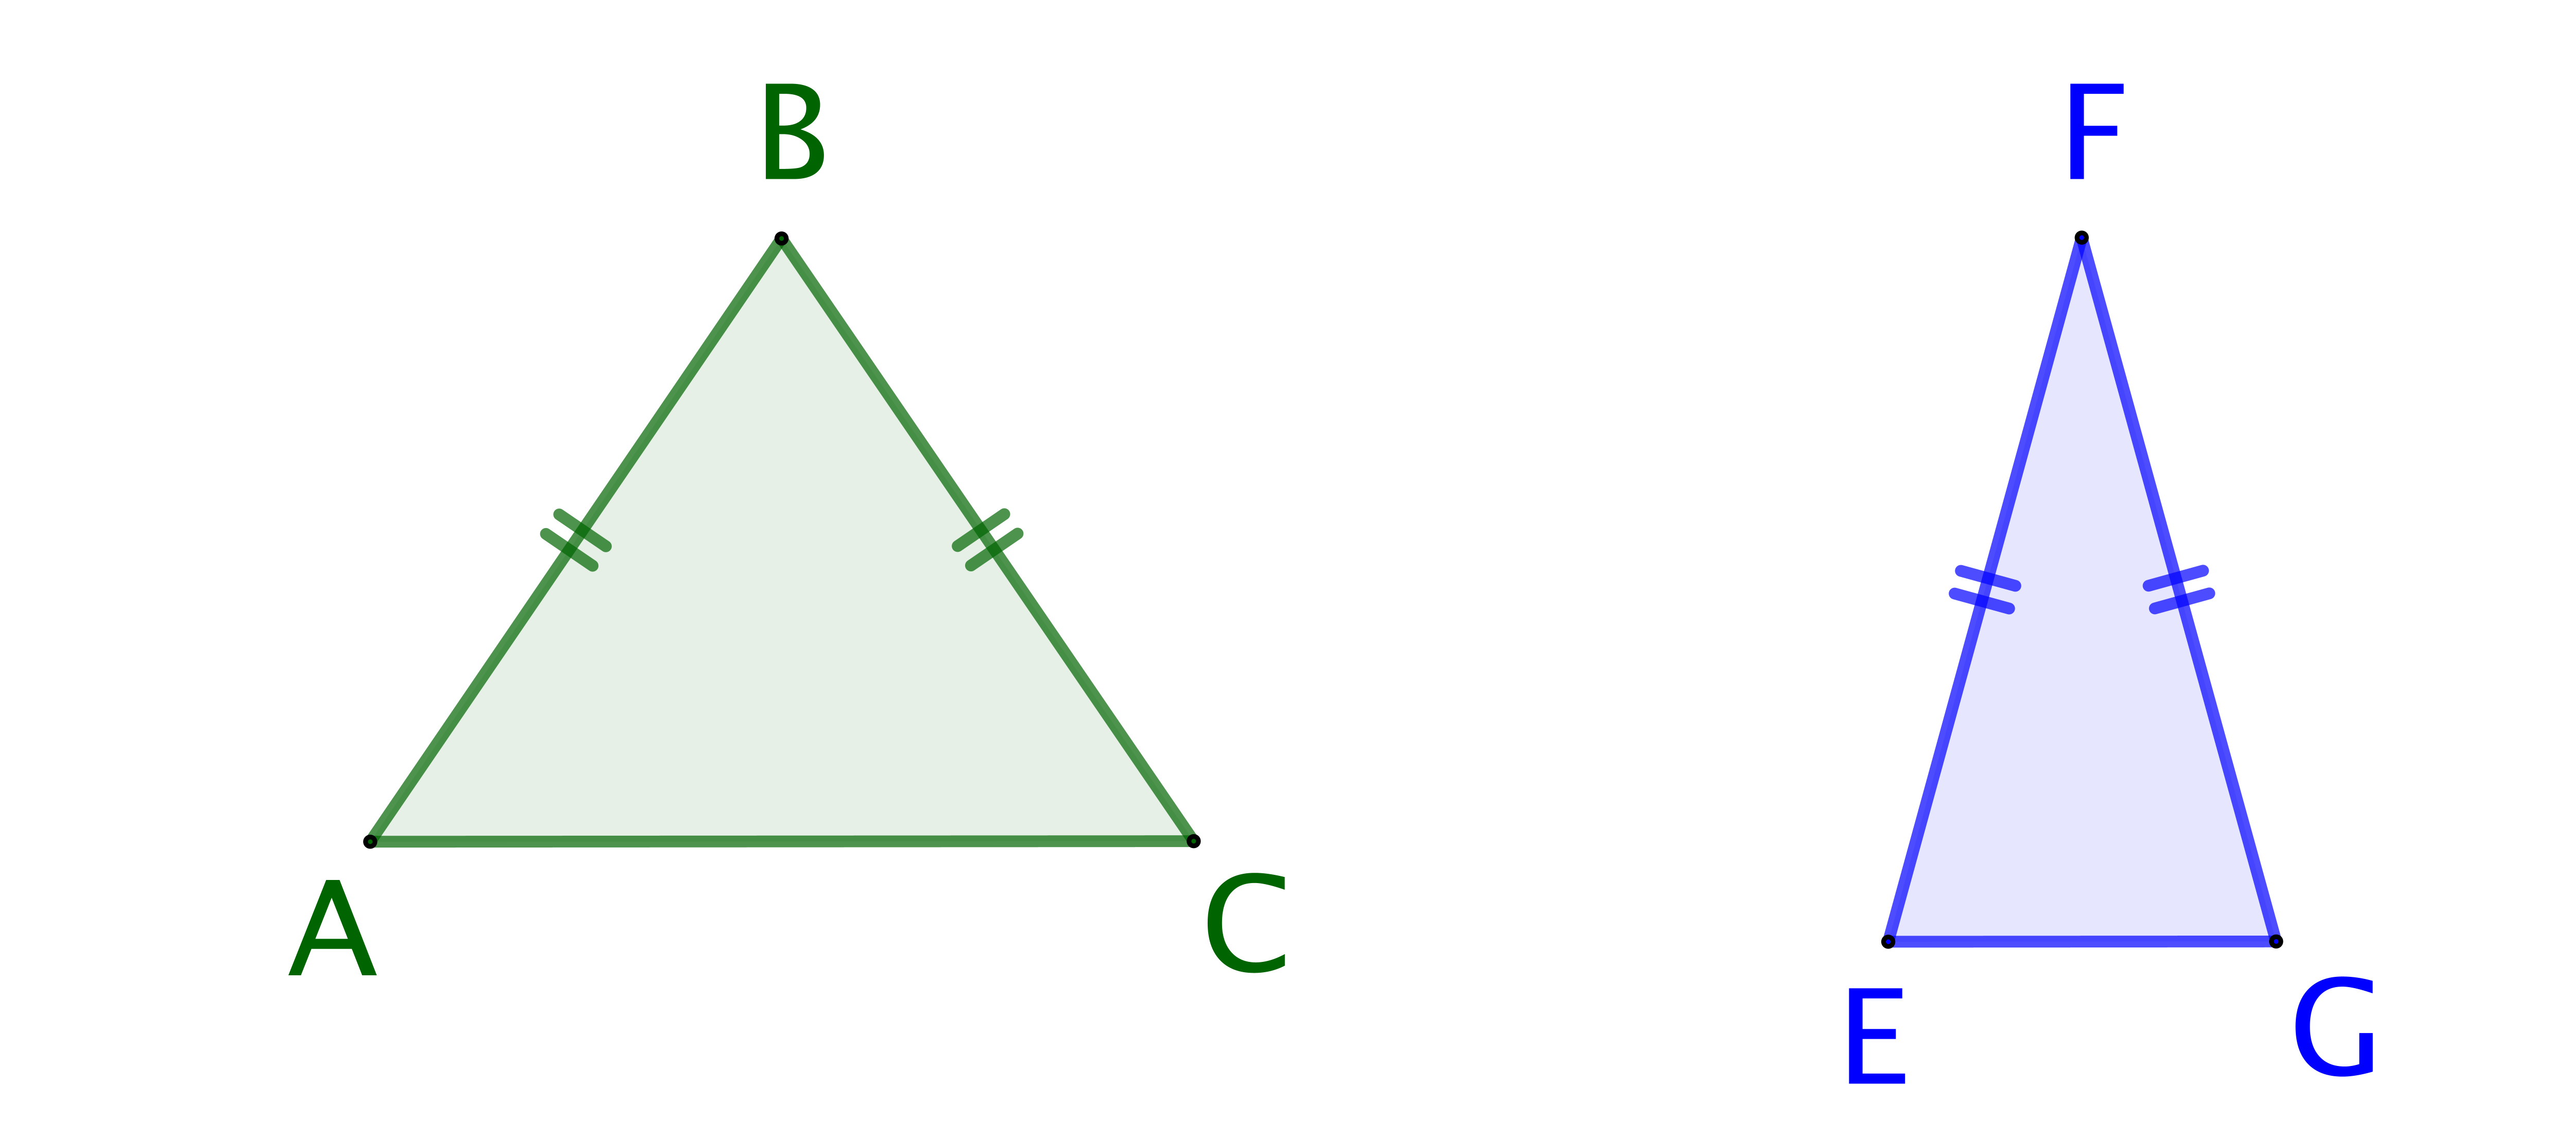
\includegraphics[scale=.4]{content/polygon/necessary-cond/2-eq-angles.png}
	\end{center}

	
	Dans nos manipulations à venir, nous fixons $A$, $C$, $E$ et $G$, tout en cherchant à bouger $B$ et $F$ de sorte à toujours avoir des triangles isocèles \og \emph{pointant} \fg\ vers l'extérieur du convexe $\setproba{P}$.
	Posons $\ell = AB$, $d_1 = AC$ et $d_2 = EG$. Comme nous ne touchons pas aux points $A$, $C$, $E$ et $G$, les nombres $d_1$ et $d_2$ sont constants.
	%
	\begin{itemize}
		\item ????

		\item ????
	\end{itemize}


%	FAUX 
%	Les deux exemples ci-dessus nous permettent de noter que si $\alpha = \anglein{ABC}$ diminue, et $\beta = \anglein{EFG}$ augmente, alors la somme des aires se rapprochent de $0$.
%	Par raison de symétrie, si on fixe $\anglein{ABC} + \anglein{EFG}$, on devine que la somme des aires est maximisée quand $\anglein{ABC} = \anglein{EFG}$.
%	Nous allons établir ceci de façon élémentaire en commençant par les calculs suivants où
%	$\ell = AB$,
%	$\mu = \frac{\alpha + \beta}{2}$ et
%	$\delta = \mu - \beta > 0$ (rappelons que nous avons supposé $\alpha > \beta$).
%
%	\medskip
%	\begin{stepcalc}[style=ar*]
%		\area{ABC} + \area{EFG}
%	\explnext*{Formule dite des sinus.}{}
%		\dfrac12 BA \cdot BC \cdot \sin \big( \anglein{ABC} \big)
%		+
%		\dfrac12 FE \cdot FG \cdot \sin \big( \anglein{EFG} \big)
%	\explnext{}
%		\dfrac12 \ell^2 ( \sin \alpha + \sin \beta )
%	\explnext*{Formules de Simpson.}{}
%		\dfrac12 \ell^2 \sin \big( \dfrac{\alpha + \beta}{2} \big) \cos \big( \dfrac{\alpha - \beta}{2} \big)
%	\explnext{}
%		\dfrac12 \ell^2 \sin \mu \cos \delta
%	\end{stepcalc}
%
%
%	\medskip
%
%	Comme $(\delta ; \mu) \in \intervalO{0}{\pi}^2$,
%	nous avons $\sin \mu \cos \delta > \sin \mu$.
%	Remplaçons alors $\alpha$ et $\beta$ respectivement par $\alpha^{\,\prime}$ et $\beta^{\,\prime}$ de telle sorte que $\alpha^{\,\prime} = \beta^{\,\prime} = \frac{\alpha + \beta}{2} = \mu$.
%	Notons que
%	$0 < \beta < \mu < \alpha < \pi$
%	(diminution de $\alpha$ et augmentation de $\beta$).
%	Deux situations se présentent à nous.
%	%
%	\begin{itemize}
%		\item Le \ngone\ obtenu ne perd aucun côté.
%		Comme la convexité est gardée, c'est gagné.
%
%		\item Le \ngone\ obtenu perd au moins un côté. La solution consiste à choisir
%		$\alpha^{\,\prime\prime} = \mu + \frac{\delta}{2}$ et $\beta^{\,\prime\prime} = \mu - \frac{\delta}{2}$
%		au lieu de
%		$\alpha^{\,\prime} = \beta^{\,\prime} = \mu$, puisque nous avons
%		$\cos \delta < \cos \big( \frac{\delta}{2} \big)$ et
%		$0 < \beta < \beta^{\,\prime\prime} < \mu < \alpha^{\,\prime\prime} < \alpha < \pi$.
%	\end{itemize}
\end{proof}


% ----------------------- %


%\begin{remark}
%	La méthode des extrema liés, rappelée dans la remarque \ref{constrained-extrema}, donne une autre justification. Voici comment faire.
%	%
%	\begin{itemize}
%		\item $\area{ABC} + \area{EFG} = \frac14 ( d_1^2 \tan \alpha + d_2^2 \tan \beta )$
%
%		\item
%		\begin{stepcalc}[style=sar]
%			4 \ell
%		\explnext{}
%			AB + BC + EF + FG
%		\explnext{}
%			2 ( AB + EF )
%		\explnext{}
%			\frac{d_1}{\cos \alpha} + \frac{d_2}{\cos \beta}
%		\end{stepcalc}
%
%		\item Pour $(\alpha ; \beta) \in \intervalO{0}{\frac{\pi}{2}}^2$, on cherche donc à maximiser $f(\alpha ; \beta) =  d_1^2 \tan \alpha + d_2^2 \tan \beta$ sous la contrainte $g(\alpha ; \beta) = 0$ où $g(\alpha ; \beta) = 4 \ell - \frac{d_1}{\cos \alpha} - \frac{d_2}{\cos \beta}$.
%
%		\item On doit avoir $\lambda \in \RR$ tel que
%    	$\pder[i]{f}{\alpha}{1} = \lambda \pder[i]{g}{\alpha}{1}$ et
%    	$\pder[i]{f}{\beta}{1} = \lambda \pder[i]{g}{\beta}{1}$
%		(méthode des extrema liés).
%
%		\item Donc
%    	$\frac{d_1^2}{\cos^2 \alpha} = \lambda \frac{d_1 \sin \alpha}{\cos^2 \alpha}$,
%		c'est-à-dire
%		$\lambda \sin \alpha = d_1$.
%		De même,
%		$\lambda \sin \beta = d_2$.
%	
%		\item ????
%	\end{itemize}
%\end{remark}








% ----------------------- %


\begin{fact} \label{nece-cond}
	Si un \ngone\ $\setproba{P}$ n'est pas régulier,
	alors il existe un \ngone\ convexe $\setproba{P}^{\,\prime}$ tel que
	$\perim{\setproba{P}^{\,\prime}} = \perim{\setproba{P}}$
	et
	$\area{\setproba{P}^{\,\prime}} > \area{\setproba{P}}$.
\end{fact}


\begin{proof}
	Le fait \ref{conv-poly} permet de considérer le problème de maximisation d'aire à périmètre fixé juste pour des \ngones\ convexes.
	Selon les faits \ref{iso-poly} et \ref{almost-reg-poly}, si, parmi les \ngones\ convexes de périmètre fixé, il en existe un d'aire maximale, alors ce ne peut être que le \ngone\ régulier.
\end{proof}
